

%=============================================================
\section{Introduction}
%=============================================================
\lettrine{T}he innovative ideas for biomimetic morphing micro aerial vehicles are promoting in the design of intelligent material structures and systems. 
%
Interests are being gained to revisit the morphing concepts, due to development of smart materials (such as piezo-electric composite). 
%
Where the structure and the actuation device form a single mechanism. 
%
Such mechanism is needed for traditional airplane. This unusual maneuvers is seen at birds. 

The comparison of the aerodynamic efficiency of gliding birds against UAVs is insightful for a better understanding of natural flight.
%
There has been an increased recognition that more attention needs to be paid to morphing wings. Wing morphing allows gulls to modulate static pitch stability during gliding \cite{Harvey2022GullMorphing}. 
%
The morphing ability of the flexible membrane wing is provided by its flexibility, which allows it to adaptively alter the shape under aerodynamic loading.
%
The aerodynamic performance modeling and flow control are drawing the interest of zoologists, biologists, and the concerned aerodynamics community.
%
As a result, these researches combine the biological theory of natural flying with aerodynamic methodologies to address MAVs based on bird endurance.

Flexible wing is a successful way for improving the aerodynamic robustness of tiny fixed wing drones operating in uncertain air situations by using a revolutionary biomimetic design.
%
The aim is to introduce a multidisciplinary approach to the study of biologically influenced flights by coupling aerodynamics, structure, and flight mechanics.
%

The birds wing aerodynamic is different in behavior compared to the conventional man-made wings as Withers \cite{Withers1981} found that the bird wings perform with low drag generally had low maximum lift coefficients, whereas wings with high maximum lift coefficients had high drag coefficients. 

Their wings are models for the construction as noise reducing application \cite{Bachmann2010}.
%
Among the studied species is the owl. They are known for their silent flight because of the features in its wings that promote smooth flow \cite{jaworski2020,geyer2016}.
% 
A thin and feather-like shapes that have a finite trailing edge thickness were designed by \citet{ananda2018aerodynamic} by using a multi-point inverse airfoil design technique in PROFOIL \cite{AirfoilDesignSoftwarefortheWeb} to design airfoil families (AS6091 to AS6099).
%
It consists of modifications in the finite trailing thickness between 4\%–6\% and can perform efficiently at the same bird Reynolds number scales ($10^4$-$10^5$).

\citet{Pabisch2010KeratinAlba} subjected the rachis to X-Ray, showing that both diameter and thickness decrease linearly from the base to the tip.

%\citet{Bostandzhiyan2008FlexuralShaft} showed that the stiffness decreases along the rachis by five and more orders of magnitude.


\begin{figure}[ht!]
\centering
\begin{subfigure}{.55\textwidth}
\centering
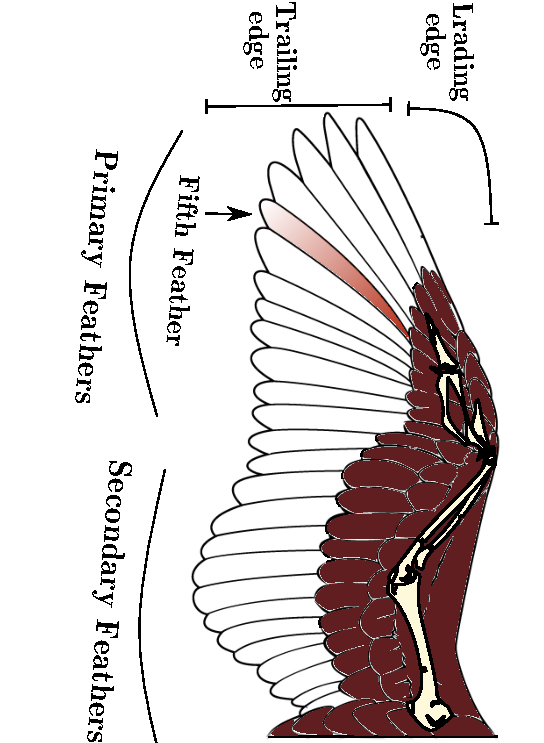
\includegraphics[width=2in, angle=90]{Figures/wing-primarySecondary.pdf}
\caption{wing anatomy}
\label{fig:anatomy} 
\end{subfigure}
\begin{subfigure}{.4\textwidth}
\centering
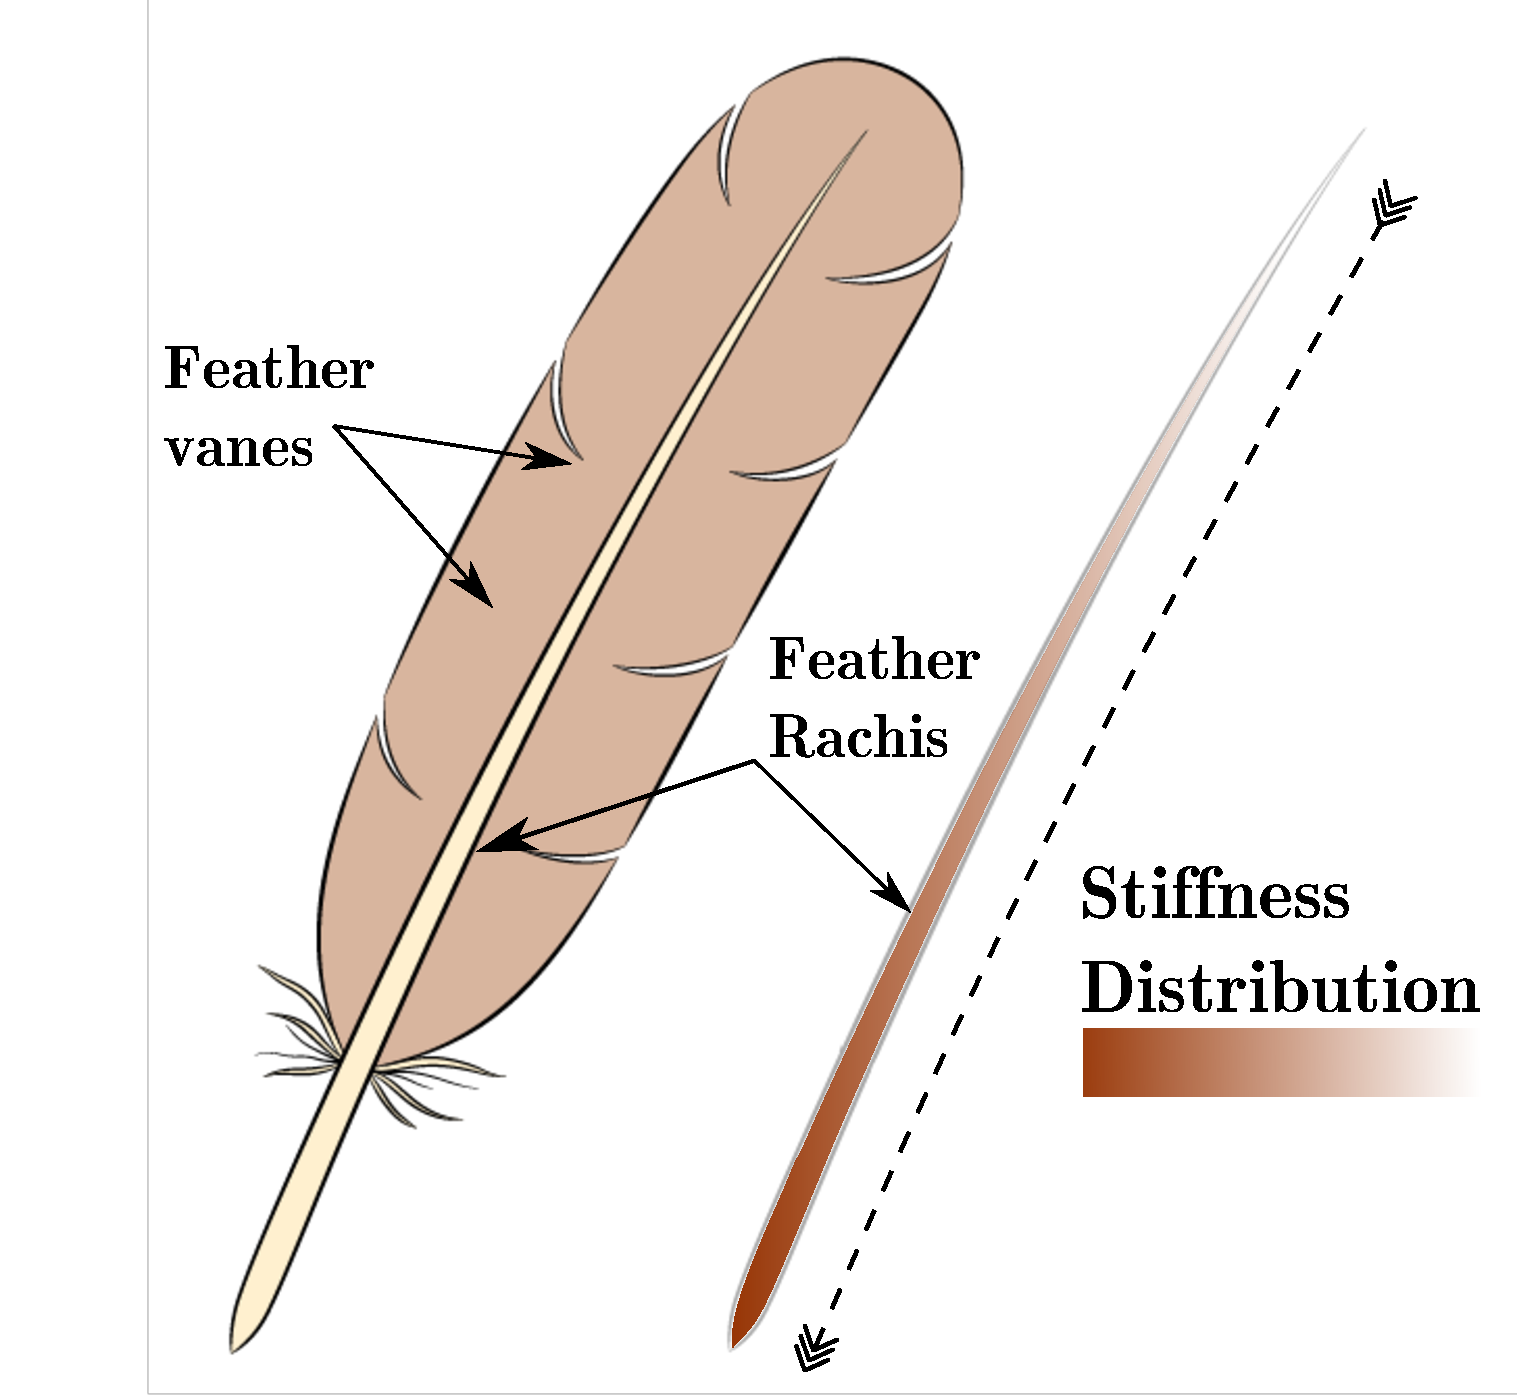
\includegraphics[width=.85\columnwidth]{Figures/shaft_drawing.pdf}
%\caption{Feather anatomy}\label{fig:anatomy} 
%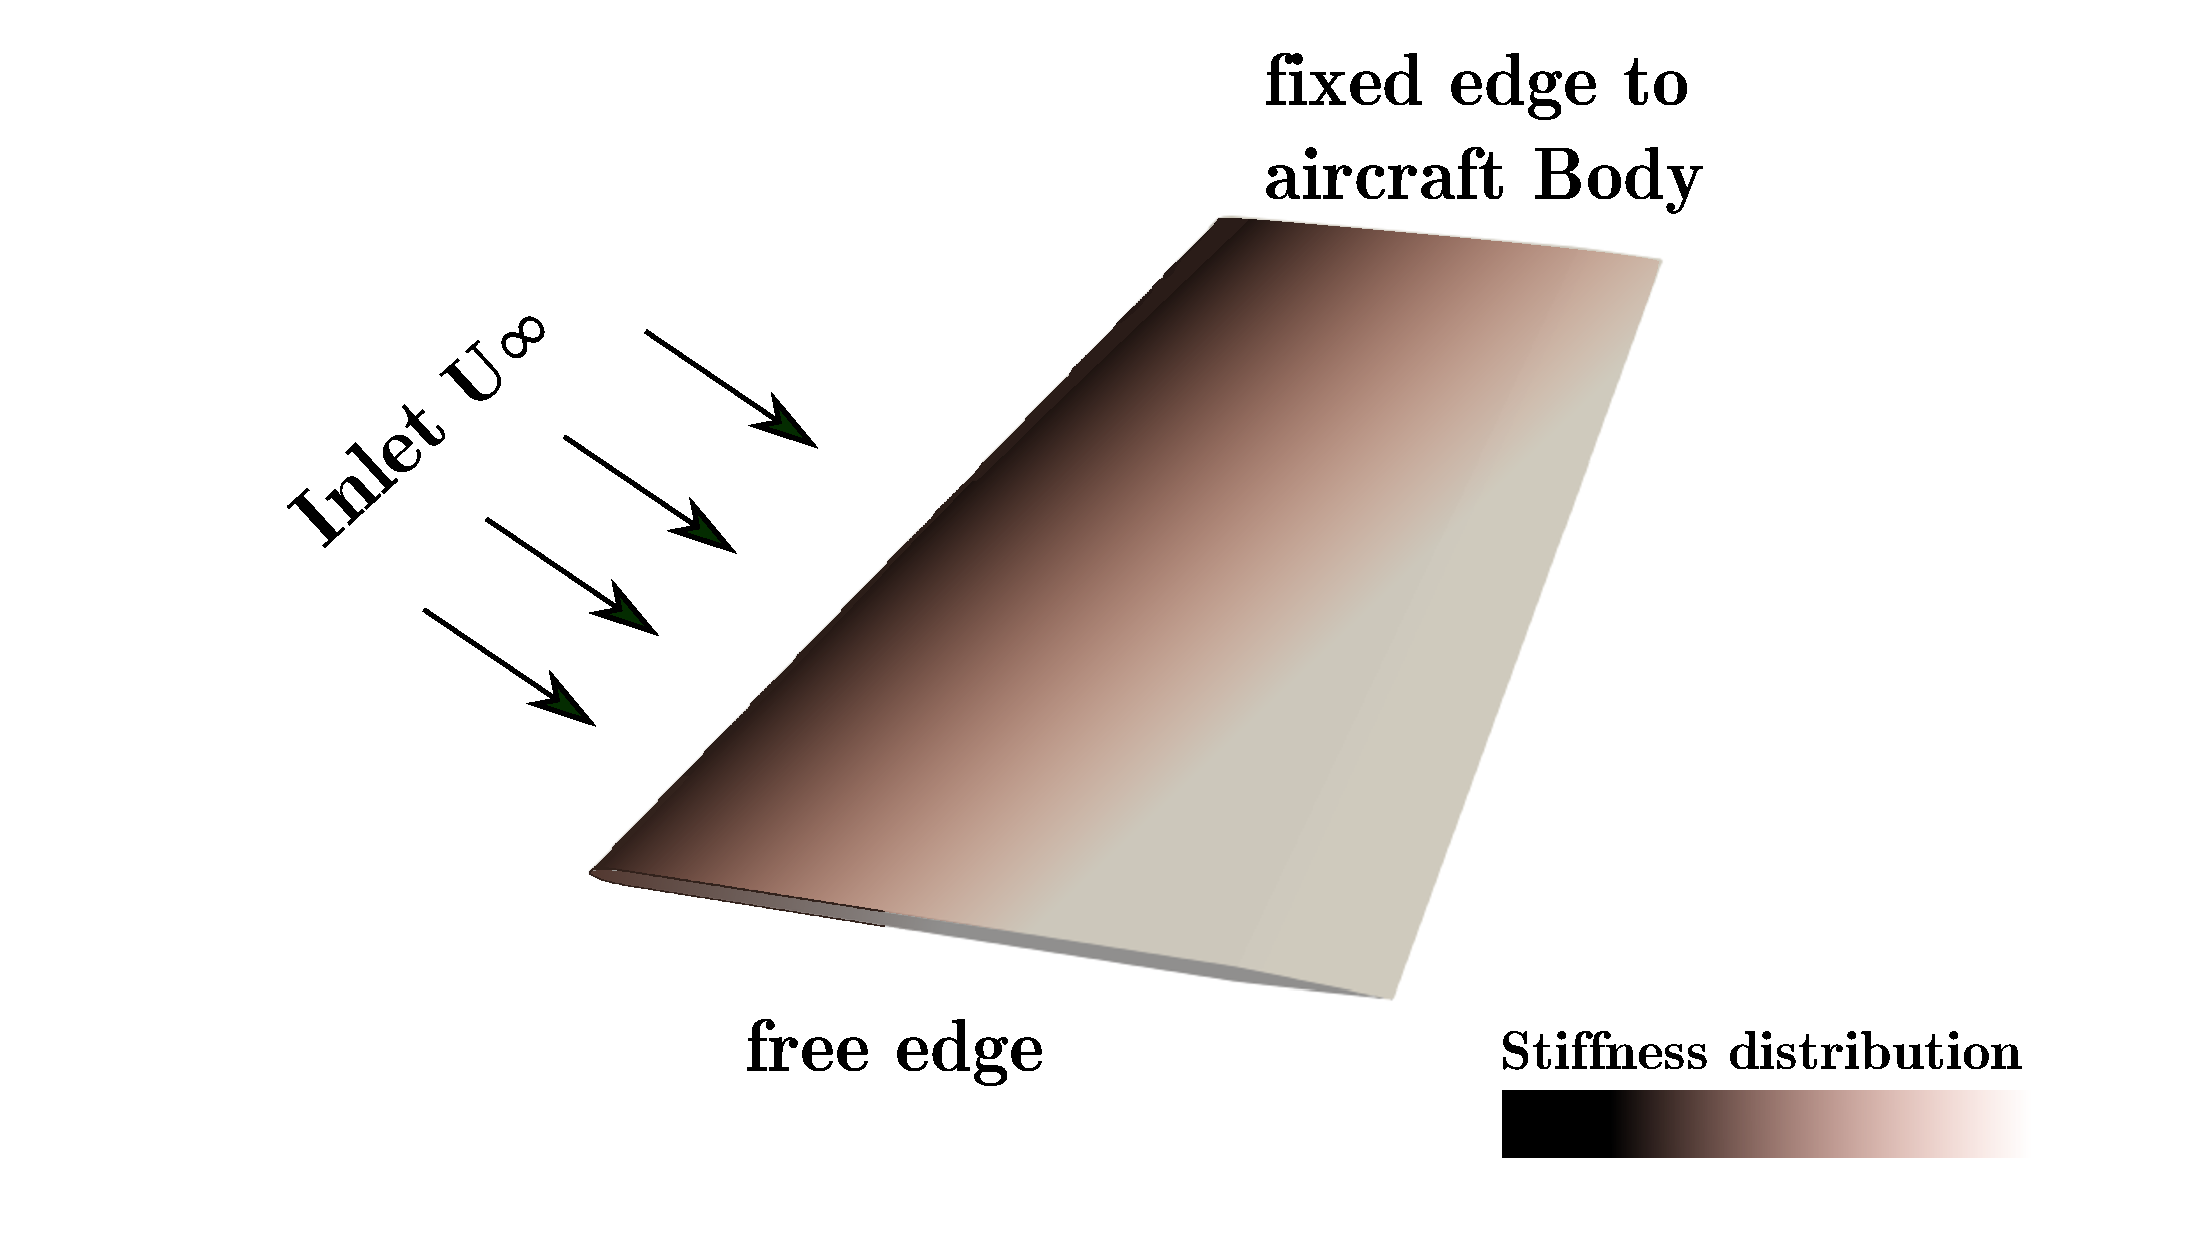
\includegraphics[width=0.49\textwidth]{Figures/plate.pdf}
\caption{Feather material properties inspiration}\label{fig:inspiration} 
\end{subfigure}
\caption{wing anatomy and Feather inspiration}
\label{fig:Ggeometry}
\end{figure}





%=======================================================
\subsection{Morphing Wings}\label{Morphing Wings}



Avian wing morphology allows inspiration for the aerostructural flow control and performance enhancement \cite{Wong2022FlexibleMorphing}. 
%
It was found that dynamically synchronizing between structural deformations and flow vortices  can improve aerodynamic performance.
%
Implementation of biomimetic approach is meant to replicate the feather effects on aerodynamic performance \cite{Hedenstrom2017}. 

%\citet{Harvey2022AControl} focused their survey on various possible controls provided by bio-inspired morphing that engineering studies could validate and incorporate to enhance flight maneuverability.
%
%Using morphing mechanisms including camber morphing techniques, wing morphing can be utilized to alter lift distributions and generate longitudinal control (cf. Fig.~\ref{fig:camberMorphing}).
%
%A deeper understanding of their control response in dynamic and turbulent environments is required, concluded the review

Early studies on experimental biology focused on the material properties testing of the biological flights such as the wings and feathers structures \cite{Bachmann2012FlexuralProperties}.



%\begin{figure}[ht!]
%\centering
%\fcolorbox{blue}{white}{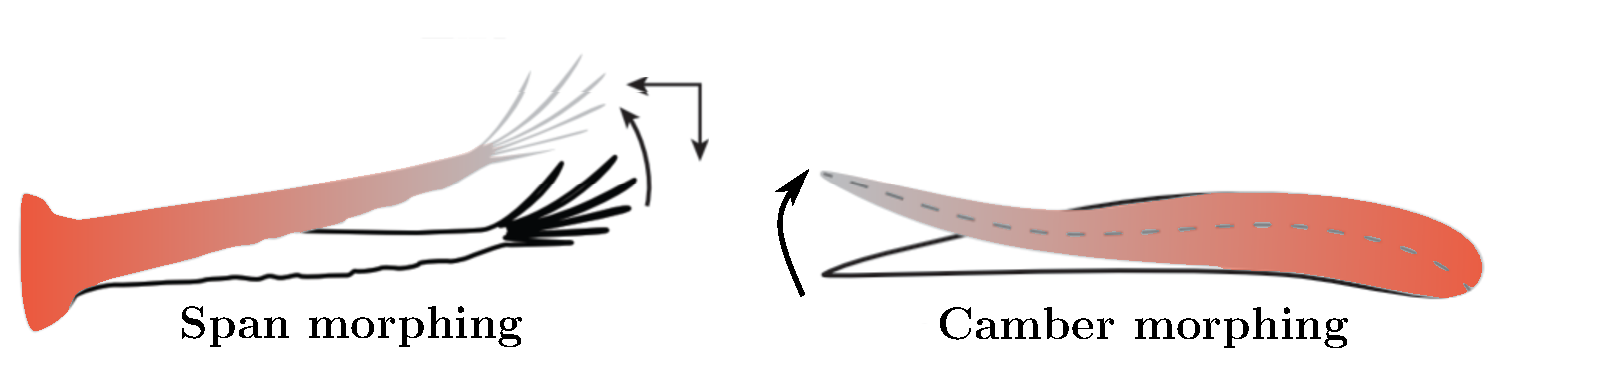
\includegraphics[width=0.9\textwidth]{figs/decambering.pdf}}
%\caption{Avian-inspired wing camber morphing spanwise cambering and chord-wise morphing \cite{Harvey2022AControl}.}
%\label{fig:camberMorphing} 
%\end{figure}

%

Although some attempts have been made to address morphing wings, much of the work in this area is limited to steady CFD predictions of the original and morphing airfoils.
%
As a first step to understanding how the flow responds to dynamic morphing flap deflection,  insightful work is presented by \citet{Abdessemed2018} using dynamic meshing to perform CFD analyses.
%
%The NACA 0012 airfoil fitted with a morphing trailing edge (TE) flap showed potential for future applications. 
%
Here it is reported that those studies neglected the dynamic aspect of the interaction between fluid and wings.
%
In these directions, a growing field of researchers studying and developing avian-inspired morphing aircraft focused on the study of the morphing wings.
%

\citet{Gamble2020b} found that the bio--inspired flexible airfoil maintained lift at Reynolds numbers below $1.5\times 10^5$, but at greater Reynolds numbers, the flexible airfoil alleviated the lift force and experienced trailing edge displacement.
%
%\cite{murayama2021flexible} in their study showed the effectiveness of flexible flaps inspired by bird feathers can improve aerodynamic robustness in low Reynolds number wings.
%
It reduces the fluctuations of aerodynamic forces in a perturbed flow behind an oscillating plate by suppressing large-scale vortex shedding. 
%
In previous work on understanding the low Re aerodynamic phenomena encountered while studying the owl-like airfoil \cite{Boughou2022} showed the unsteadiness of the aerodynamic coefficients.
%
The aero-structural response to the aerodynamic load is the motive behind the work presented in this paper.

The role of feather morphing hasn't been thoroughly investigated, and its impact on aerodynamics is unknown. 
%
The aero-structural response of a flexible airfoil designed using biologically inspired structural and material data from feathers requires studies that concentrate on evaluating aerodynamic load and the aero-structural features in turbulent situations.
%
In the current study on bio-inspired flexible wings, we aim to make use of existing research in the field of experimental biology and complete several engineering objectives. 

%\begin{figure}[h!]
%    \centering
%    \fcolorbox{blue}{white}{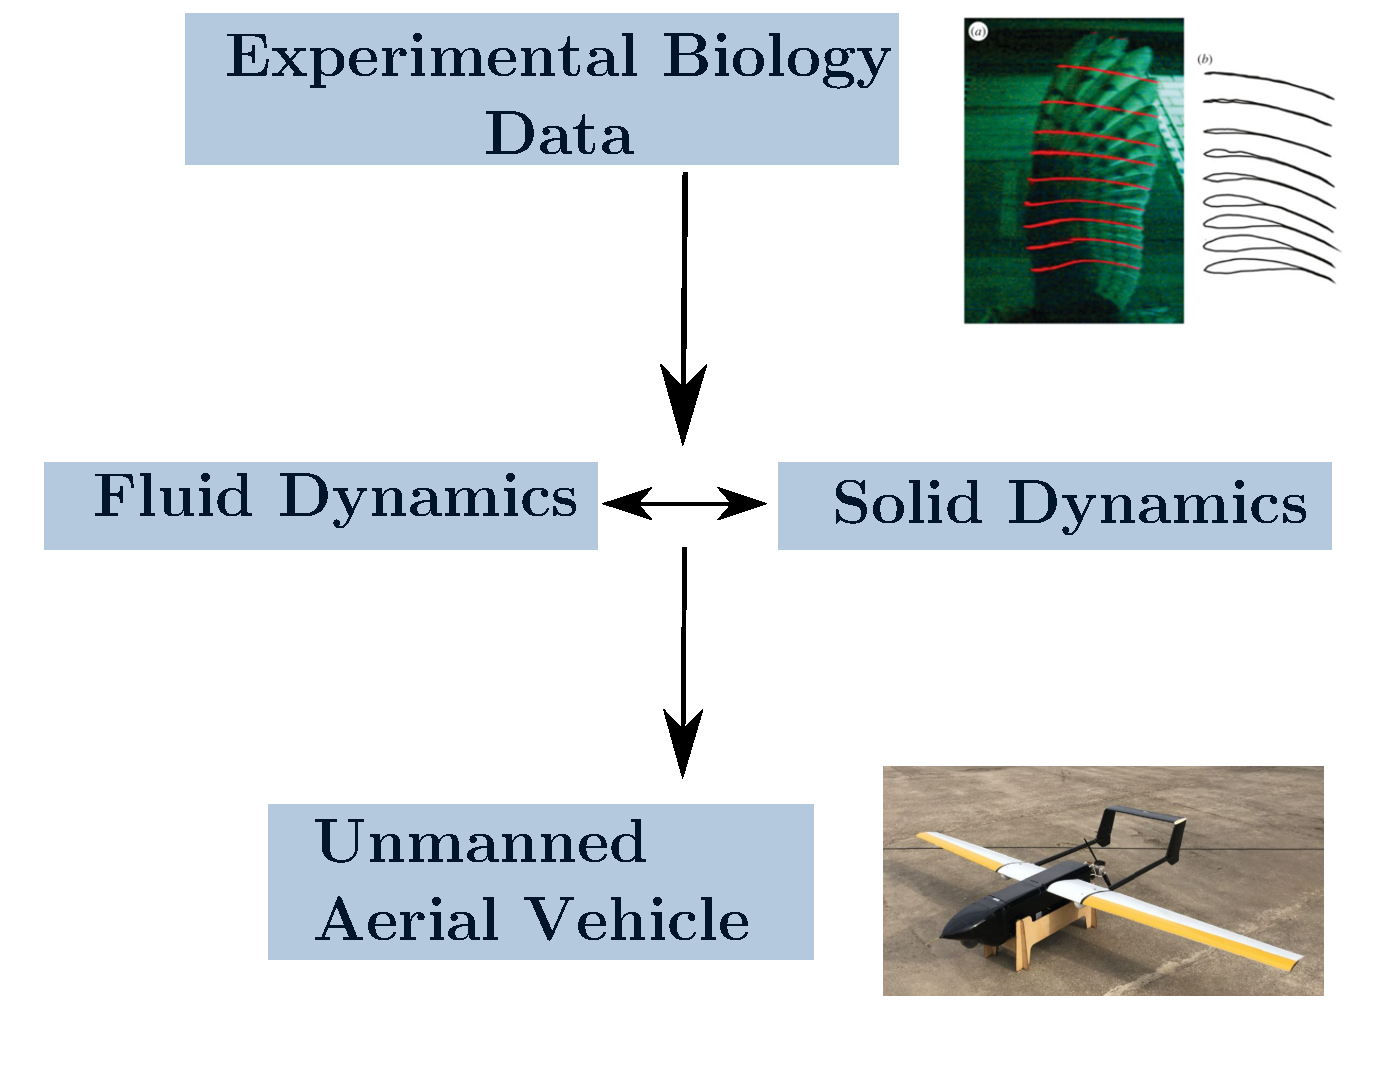
\includegraphics[width=0.4\textwidth]{Figures/bioengineering.pdf}}
%    \caption{Work Flow for Bio inspired Flexible wing}
%    \label{workflow}
%\end{figure}

First, we examine bio-inspired structure requirements  necessary to capture both flow field and structural analysis. 
%
Unlike most of the state-of-the-art nonlinear aeroelastic frameworks that use the geometric nonlinear beam-based model, here a finite volume solid mechanics is implemented.

Computational modeling can provide a way to develop predictive relationships between morphological traits and their impact on aerodynamic performance through a series of flexibility conditions that will be computed using Fluid-Structure interaction (FSI).
%
The primary objectives of evaluations is to investigate the dynamic interaction between Low Re aerodynamic flow and Flexible-Biomimetic NACA6409 as earlier recommended in Ref \cite{gamble2020b} at an angle of attack $15^{\circ}$.
% 

%
Following the work of \citet{Gamble2020b}, we use simplified bird airfoil as the basis for this computational study and a Young's modulus $\mathcal{E}$ of 2.5 GPa chordwise stiffness that may allow feather replication with a constant Young's modulus.

By doing so, this numerical testing of both the biological and the replicated flexible trailing edge verifies that these
bio-inspired techniques can be reproduced in an engineering configurations.


\newpage
%=============================================================
\section{Material and Methods}
%=============================================================


%========================================
\subsection{Avian-like wing $\&$ Feather replication}
%=======================================

Bird wings cross section (airfoils) are of special profiles.
%
A thin and feather-like shapes that have a finite trailing edge thickness are considered for the current work. 
%
Different biological flight aspects are inspired and mimicked. 

\subsubsection{mechanical properties inspiration}

Previous studies concluded that the Young's modulus can be adjusted along the chord so that the equivalent the stiffness distribution replicates the feather.

It's shape was modelled as a cone \cite{Lingham-Soliar2017MicrostructuralFeathers}, which thickness decreases linearly from the leading edge to the tip. This would provide a first insight on modelling material properties.

As \citet{Bachmann2012} reported in their experimental biology work, two parameters are mainly affecting flexibility of feathers.
%
They used two different methods (two-point bending test and Nanoindentation) to determine the Young's modulus of feather keratin of barn owl that provided similar results.
%
They provided in various biological experiments on the rachis, different material properties such as the Young's modulus $\mathcal{E}$ (Modulus of elasticity) and second moment of area $\mathcal{I}$ (second Moment of inertia). 
%
Therefore, the flexural stiffness of the whole rachis is mainly sensitive to the cross-sectional geometry rather than by the Young's modulus of the keratin.
%
This latter ($\mathcal{I}$) dominates over the bending stiffness behavior along the feather length.

The variation in Young’s modulus along the shaft length is provided Experiment by \citet{Bonser1995TheKeratin}. 
%
The feather shaft properties are examined by smaller samples that are analyzed to determine the variation of the tested properties along the feather length.
%
The measurement pattern shows to fit a linear regression (see Fig.\ref{fig:segments}).
%
Therefore, the variation of Young's modulus is supplied to  the model as an expression of linear function.
%
For the stiffness, it decreases along the feather by five and more orders of magnitude.
%
Therfore, the tip almost vanishes in stiffness \cite{Bostandzhiyan2008FlexuralShaft}.
%
Same trend of increasing in Young's modulus along the rachis was confirmed in \cite{Cameron2003YoungsFeathers}.


\begin{figure}[ht!]
\centering
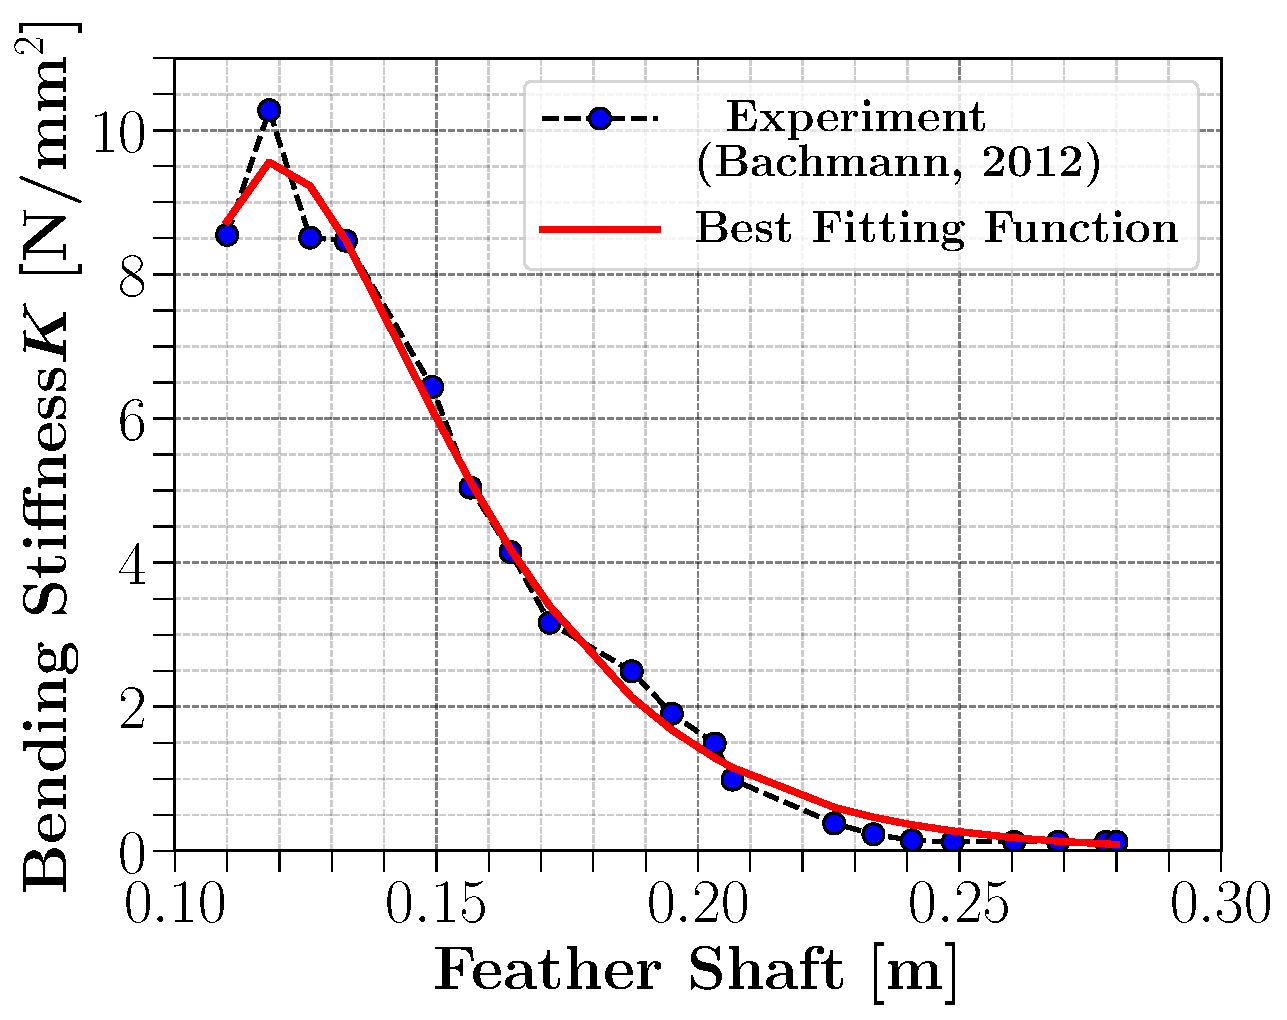
\includegraphics[width=0.4\textwidth]{figs/Bending-distribution.pdf}
\caption{Stiffness variation along the shaft length; Fitting with data from Ref \cite{Bachmann2012FlexuralProperties}}
\label{fig:stiffness}
\end{figure}



%\begin{table}[ht!]

%\caption{\label{Properties} Mechanical Properties }
%\centering
%\begin{tabular}{@{}lll}
%\hline
%\bf{Characteristic} & \bf{Nomenclature} & \bf{Value} \\
%\hline
%Length & $\mathbf{b}$ & 0.28 m\\
%Young Modulus & $\mathcal{E}$ & 2.5-0.25 GPa\\
%Poisson ratio & $\nu$ & --\\
%Shear modulus & $\mu$& --\\
%Bending Stiffness&$\mathcal{K}$&--\\
%\hline
%\end{tabular}

%\end{table}



%=========================================================

\subsection{Numerical Methods}

%=========================================================


%========================================
\subsubsection{rigid and flexible part inspiration}
%========================================
As part of the validation of this work, this model builds upon the previous work of \citet{Gamble2020b} in which the modelling of feather-like airfoil is done by considering it as two part segments: rigid part and flexible one.

From previous studies, bird-like low Reynolds number airfoils \cite{Boughou2022NumericalAirfoils} showed to perform as a high lift airfoils.
%
Some of conventional NACA airfoils exhibits as such high lift in terms of aerodynamic performance.
%
The choice of NACA6409 for current investigations meets the bird wing cross-section analogy.




The rachis' structure in current study is mimicked with a wing cross section flexible at the trailing edge (cf. Fig.~\ref{fig:segments}).
%
Anatomy of bird airfoil considering rigid and flexible segments; NACA6409 airfoil segments (40\% ) rigid and (60\%) flexible denoted $\mathcal{L}$

\begin{figure}[ht!]
\centering
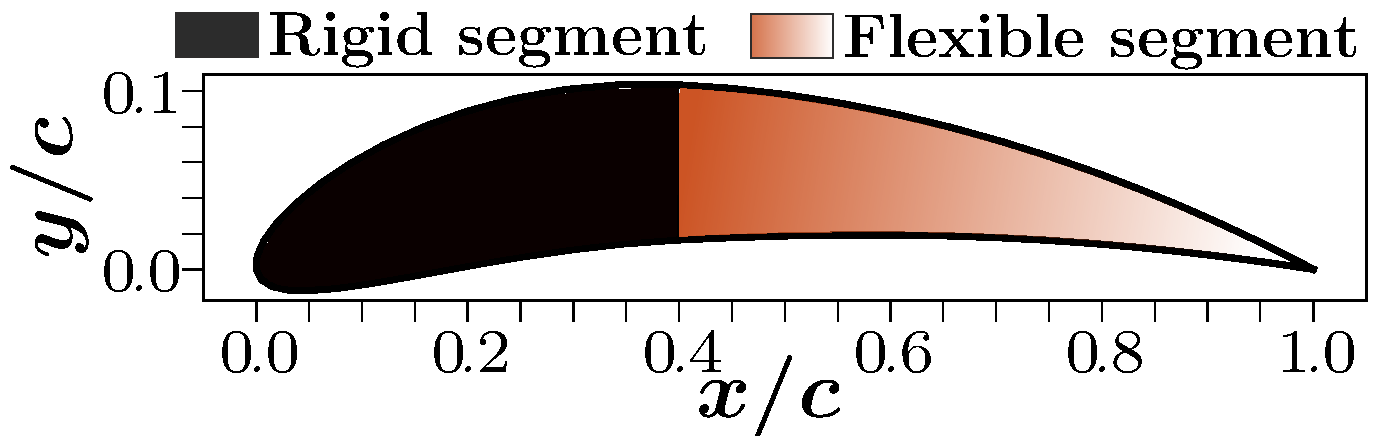
\includegraphics[width=0.5\textwidth]{figs/segments_airfoil.pdf}
\caption{Anatomy of bird airfoil considering rigid and flexible segments; NACA6409 airfoil segments (40\% ) rigid and (60\%) flexible denoted $\mathcal{L}$}
\label{fig:segments}
\end{figure}




%=========================================================

\subsubsection{Wing Models}

%=========================================================
 
Airfoil configuration and computational mesh used for the fluid–solid interaction problem is displayed in Fig.~\ref{fig:Ggeometry}.
%
As shown in Fig.~\ref{fig:Griddomain}, the computational domain is built with a structured grid using the ANSYS multi-blocks grid ICEM tool, with the appropriate boundary conditions.
%
The mesh plane is extruded in span wise direction with a one cell.
%
The mesh is fine in order to avoid high aspect ratio cells within the domain.
%
The next section \ref{sec:results} outlines the preliminary resulting data assessed in multiple stages of the study of the NACA6409 airfoil (cf. Fig.~\ref{fig:6409}) at Reynolds number of $10^5$ to $5\times 10^5$ considering a rigid segment of 40\% and flexible segment 60\% chord length (cf. Fig.~\ref{fig:airfoilSegments}).
The NACA6409 airfoil is defined to have a max camber of $ 6\%$ at $39.6\%$ chord at the location where the flexible trailing edge

\begin{figure}[ht!]
\centering
\begin{subfigure}{.5\textwidth}
\centering
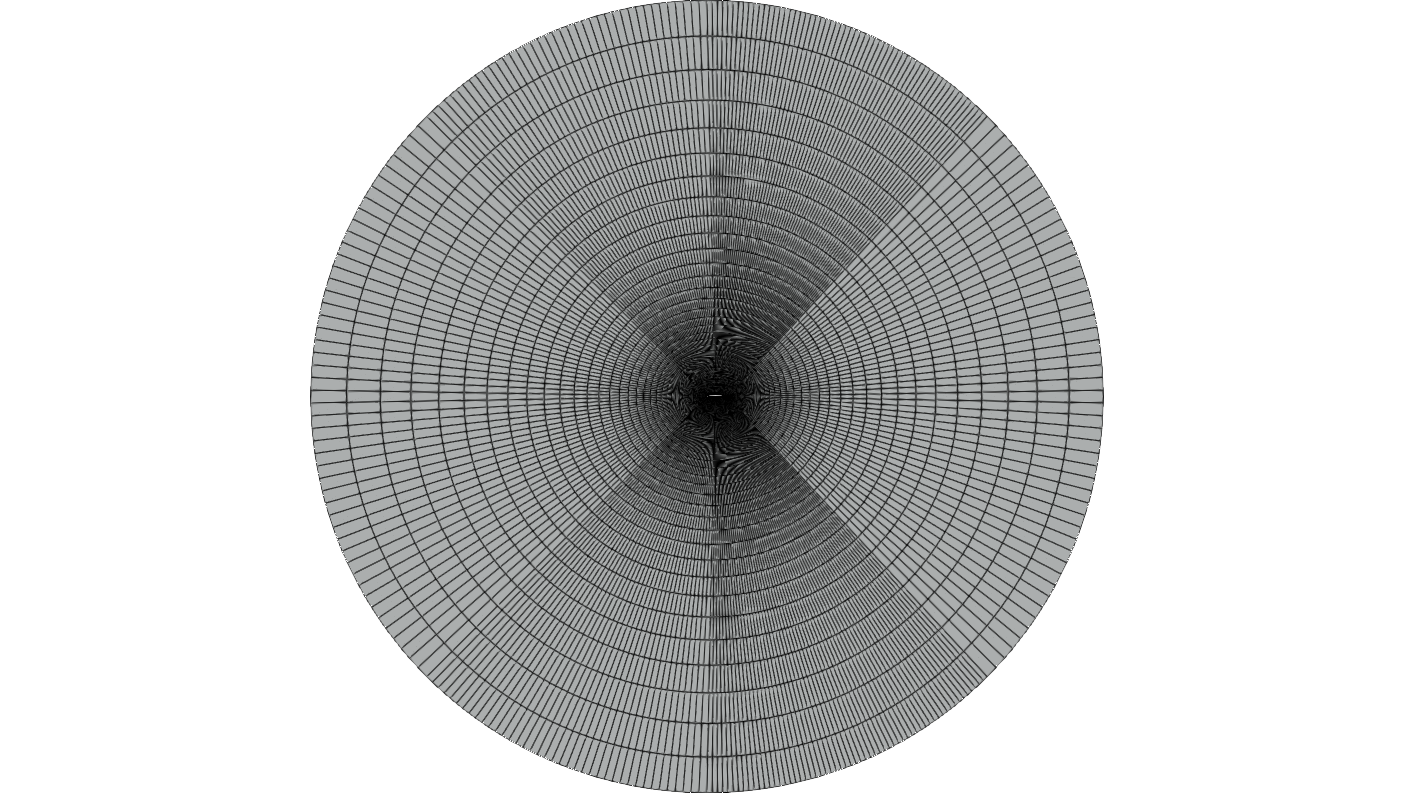
\includegraphics[width=4in]{Figures/Grid.png}
\caption{\label{fig:Griddomain} Grid domain}
\label{fig:airfoildesigna}
\end{subfigure}
\begin{subfigure}{.4\textwidth}
\centering
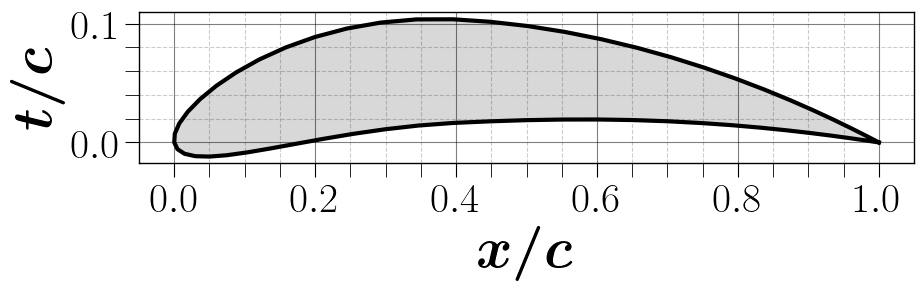
\includegraphics[width=.6\columnwidth]{figs/naca6409_airfoil.png}
\caption{\label{fig:owl}NACA6409}
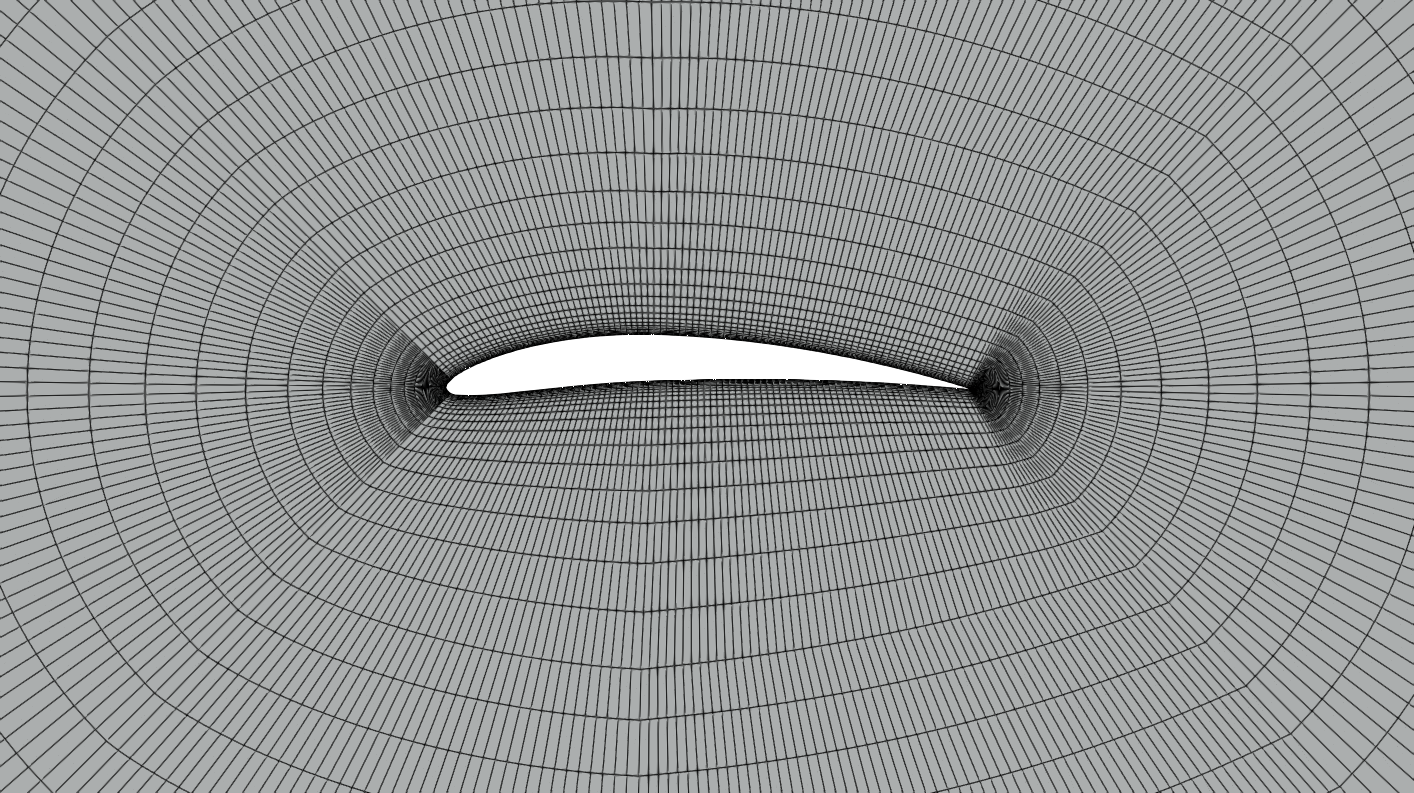
\includegraphics[width=.6\columnwidth]{Figures/airfoilGrid.png}
\caption{\label{fig:6409}Grid around airfoil surface}
\end{subfigure}
\caption{Computational fluid domain and wing profile}
\label{fig:Ggeometry}
\end{figure}
%

\begin{figure}[ht!]
\centering
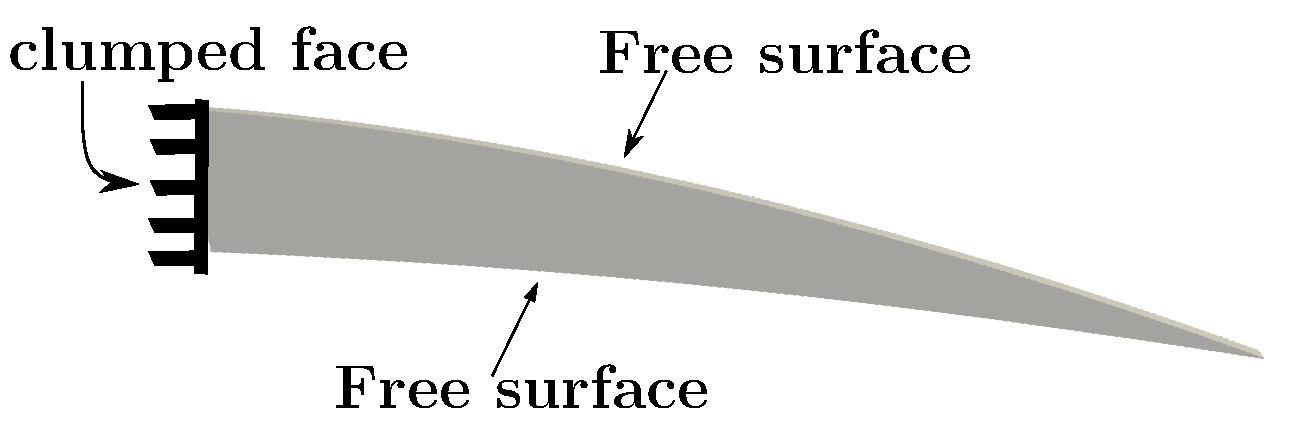
\includegraphics[width=0.5\textwidth]{Figures/naca6409_solid.pdf}
\caption{ Boundary conditions for the flexible segment; NACA6409 airfoil segments (60\%) flexible }
\label{fig:segments}
\end{figure}



%=========================================================
\subsubsection{Fluid-Structure Interaction}
%=========================================================

Fluid-Structure Interaction (FSI) is defined as fluid flow applying forces to solid bodies and the solid’s dynamic response changes the surrounding flow field. 
%
This is achieved through transferring information between the interfaces of the fluid and solid.
%
For the aero-elastic analysis of large-deformation structures, nonlinear structural model is developed, since the current biological materials do not exhibit the linear elastic behaviour.
%
To investigate how the structure responds to aerodynamic load, the governing equation for Neo-Hookean hyper-elasticity as described in \citet{Wiggins1998ComputationalInelasticity} is implemented.

With considering: 
    \begin{equation}
        \mu= \frac{\mathrm{E}}{2(1+\nu)}
    \end{equation}
    \begin{equation}
        \mathcal{K}= \frac{\nu*E}{((1.0 + \nu)*(1.0 - 2.0*\nu))} + \frac{2}{3}\mu
    \end{equation}

%

FSI Simulations are performed with an open-source finite volume toolbox for solid mechanics and fluid-solid interaction simulations.
%
The finite volume method described for orthotropic bodies subjected to large strains and large deformations with consideration of updated Lagrangian finite volume solver \cite{Tukovic2014} is implemented in the FSI method described in this work.
%
To resolve the well-known computational aerodynamics and aeroelastic airfoils, the FSI procedure is combined with the turbulence model k-$\omega$ SST and large deformation updated Lagrangian finite volume structure solver \cite{Cardiff2018}.

\begin{figure}[ht!]
\centering
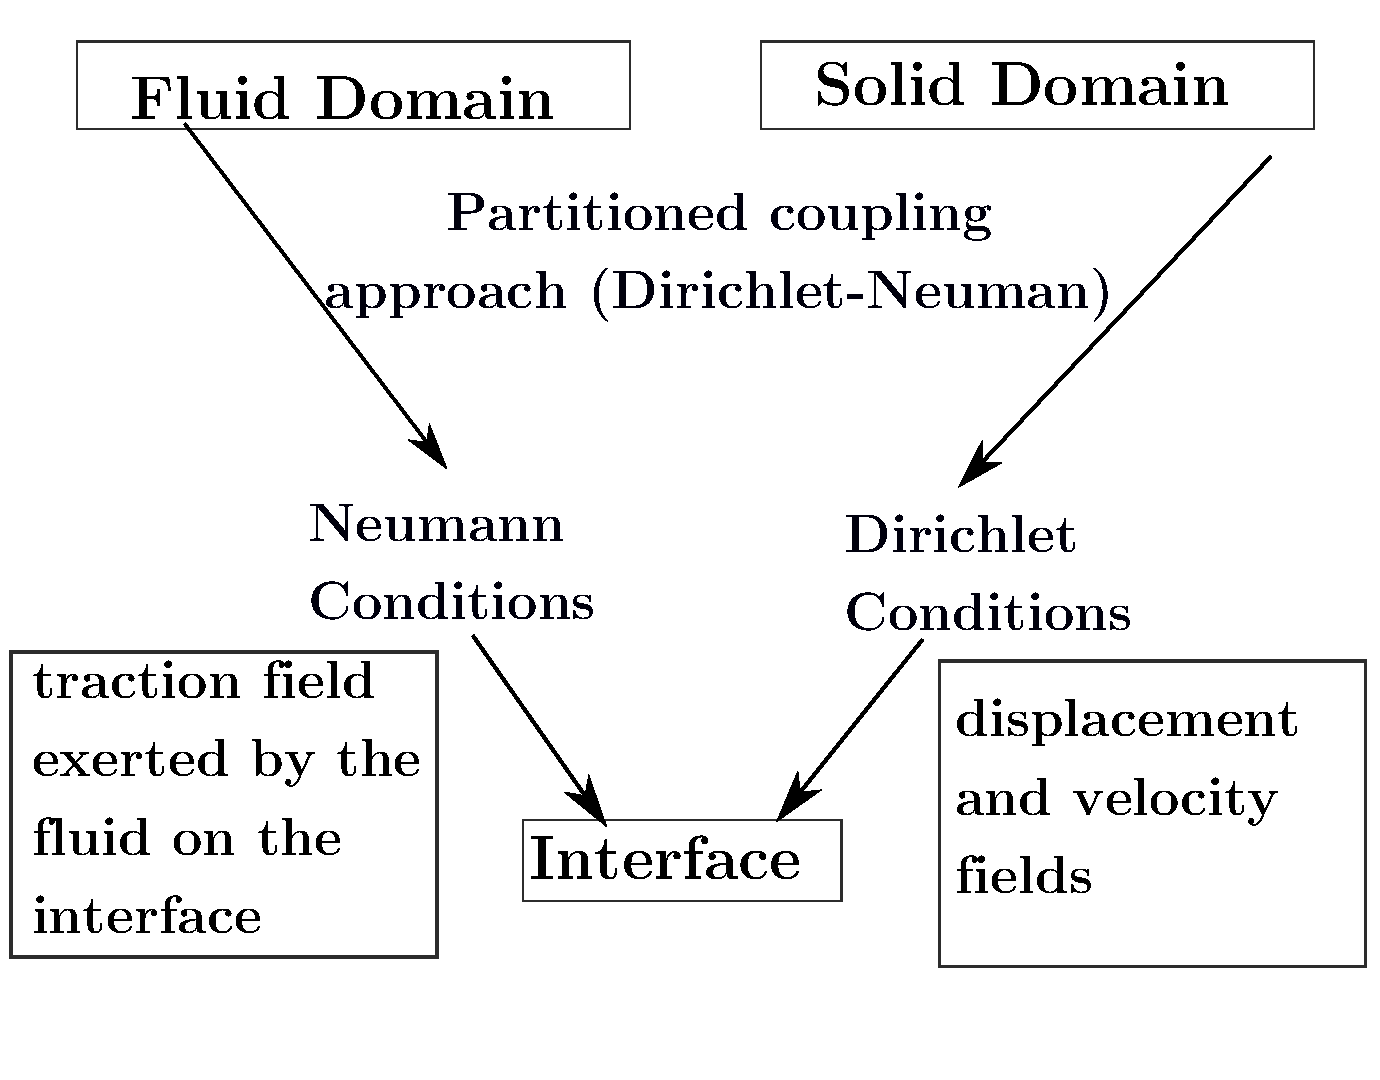
\includegraphics[width=0.45\textwidth]{Figures/FSI.pdf}
\caption{FSI Coupling procedure}
\label{fig:airfoilSegments} 
\end{figure}





%=============================================================
\section{FSI Analysis}
\label{sec:results}
%=============================================================




%=============================================================
\subsection{Flow Field}
\label{sec:flowField}
%=============================================================

%
Comparison of the CFD results is done by quick assessment using XFoil panel method \cite{Drela1987}, it shows the stall of lift coefficient near an angle of attack 15 $^\circ$. 
%
The convergence of the steady state solution of the lift coefficient  at and AOA 15 is shown at the Fig. \ref{fig:lfitCoe}





\begin{figure}[ht!]
\centering
\begin{subfigure}{.45\textwidth}
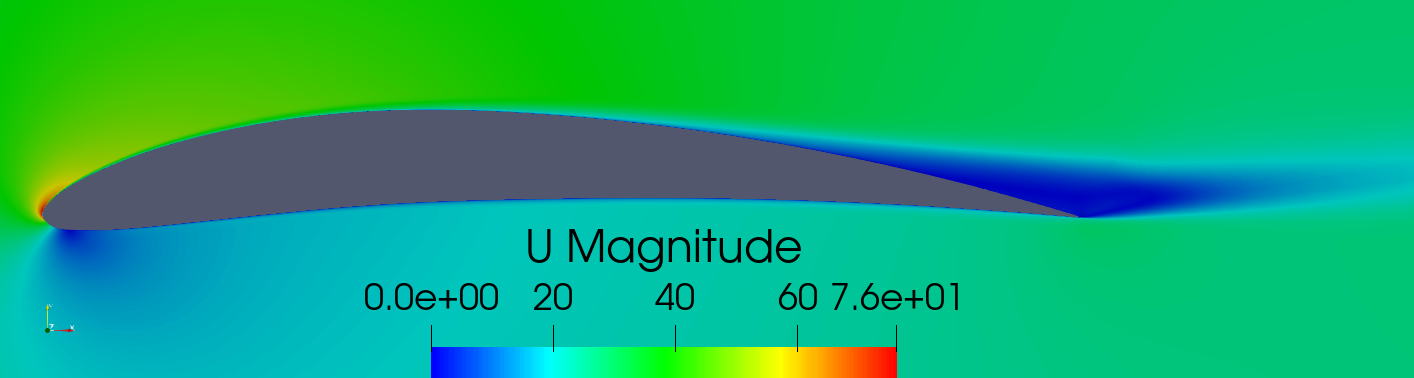
\includegraphics[width=0.99\columnwidth]{Figures/VelocityContour.png}
\caption{Velocity contour of flow field at $\mathcal{R}_e=2\times10^5$}
\label{fig:velocitycontour}
\end{subfigure}
\begin{subfigure}{.45\textwidth}
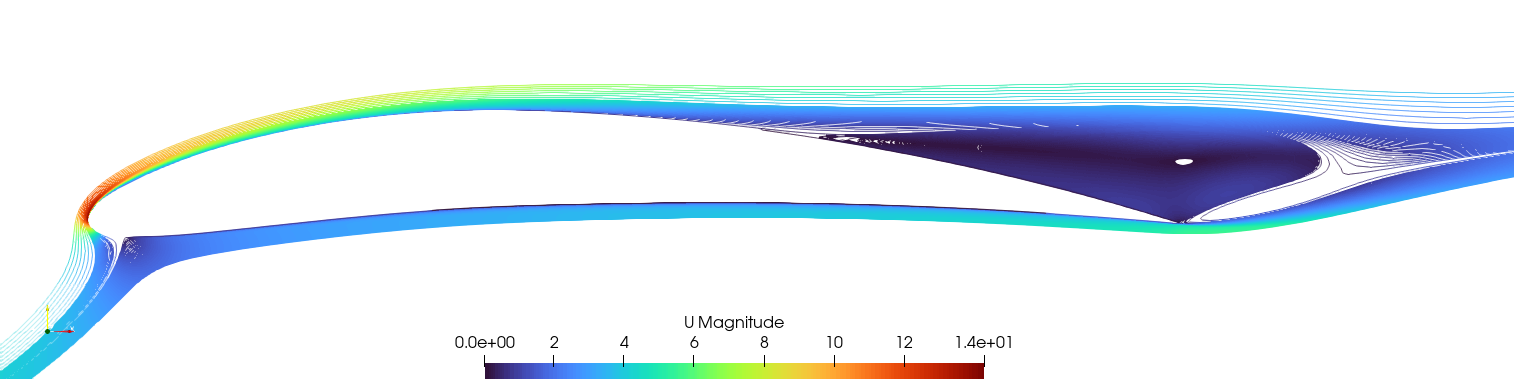
\includegraphics[width=0.99\columnwidth]{figs/velocityContours2.png}
\caption{Streamlines around airfoil obtained at $\mathcal{R}_e=2\times10^5$}
\label{fig:streamlines}
\end{subfigure}
\caption{\label{fig:history} Highlight of separation bubble at $\Rey =5\times10^5$ }
\label{fig:history}
\end{figure}

%
Within stall region, the flow begins to separate over the upper surface. 

\begin{figure}[ht!]
\centering
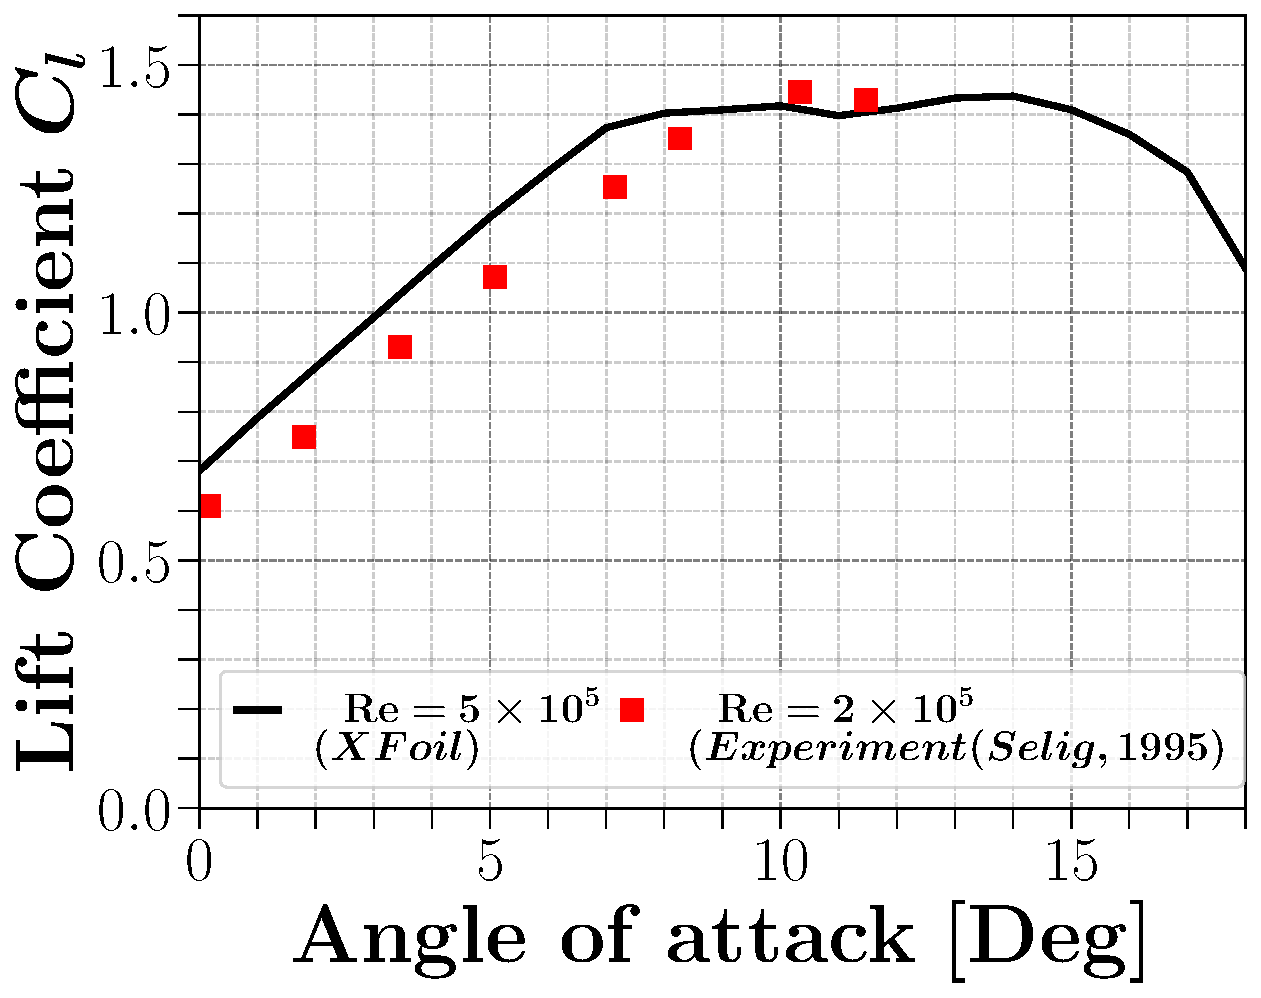
\includegraphics[width=0.4\textwidth]{figs/liftCoeff.pdf}
\caption{Lift coefficient of NACA6409 airfoil at $\boldsymbol{\Rey$ = 5 $\times 10^5}$}
\label{fig:lfitCoe} 
\end{figure}

For reasons of ensuring flow development, the flow field around the NACA6094 at a $\mathcal{R_{\mathbf{e}}} = 5 \times 10 ^5$ is studied.
%
At the angle of attack $15^{\circ}$ is near-stall conditions where the flow begins to separate over the surface.
%
Which is the reason behind the choice of running the simulation at $15^{\circ}$.
%
The figure \ref{fig:lfitCoe} shows the non-dimensional time history of the aerodynamic lift coefficient ($\mathcal{C}_\mathscr{l}$) at the angle of attack $15^{\circ}$.
%
The resulting $\mathcal{C}_\mathscr{l}$ is in agreement with in the experimental works of \citet{Selig1995} at University of Illinois at Urbana-Champaign (UIUC) wind tunnel tests.


\begin{figure}[ht!]
\centering
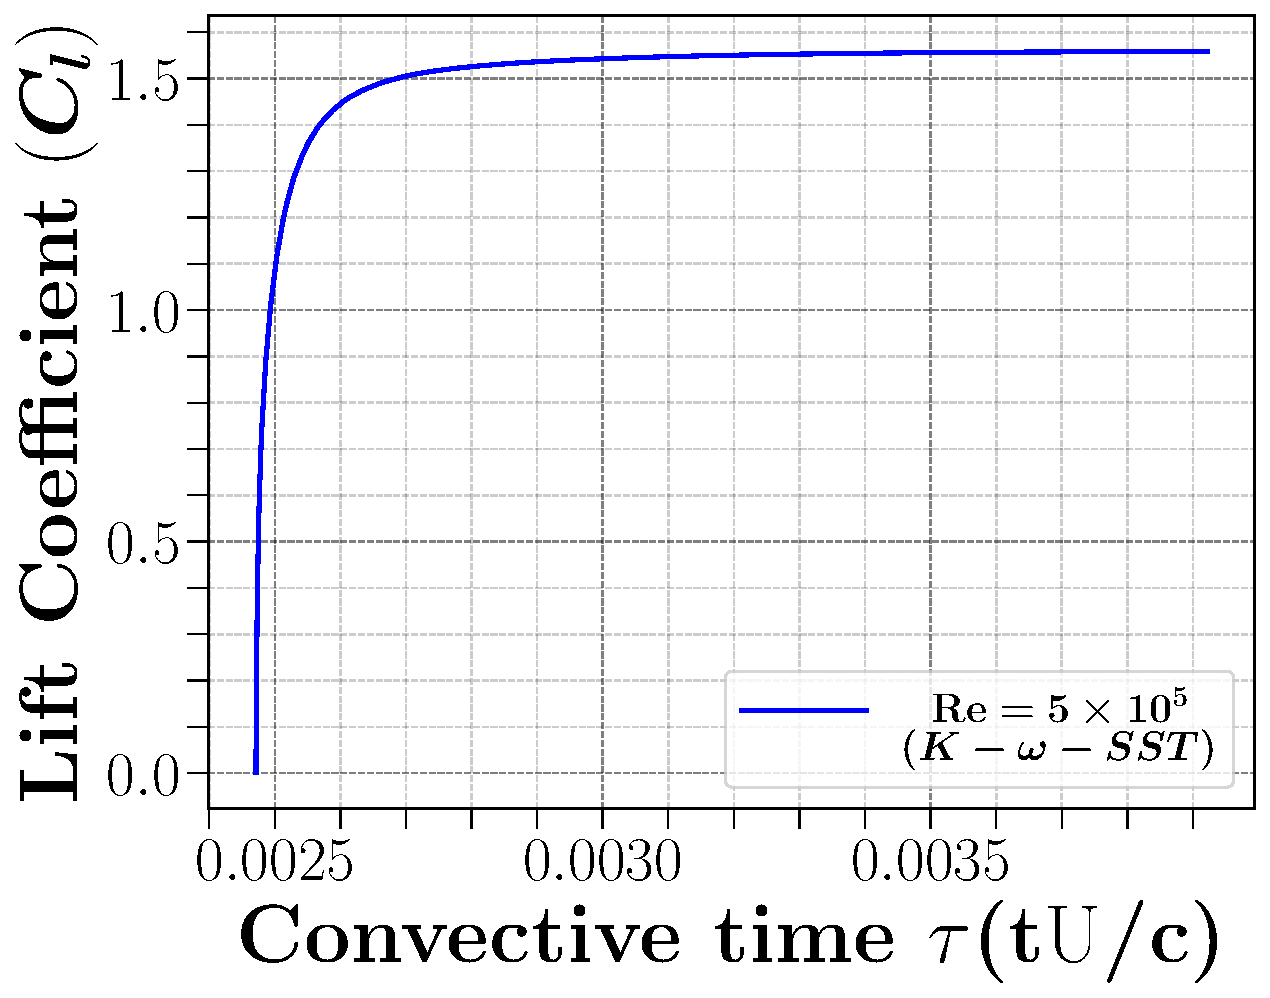
\includegraphics[width=0.4\textwidth]{figs/LiftCoeAngle15.pdf}
\caption{Lift coefficient of NACA6409 airfoil at the angle of attack $15^{\circ}$ and $\boldsymbol{\Rey$ = 5 $\times 10^5}$}
\label{fig:lfitCoe} 
\end{figure}







%For the unsteadiness of the flow reasons, the effect of the coupling time of fluid and structure calculations is also investigated for the independence from the timing.




The difference of pressure over the upper and lower surfaces of the airfoil  shown in the figure \ref{fig:Cpcontour} will be applied in the solid surface.


\begin{figure}[ht!]
\centering
    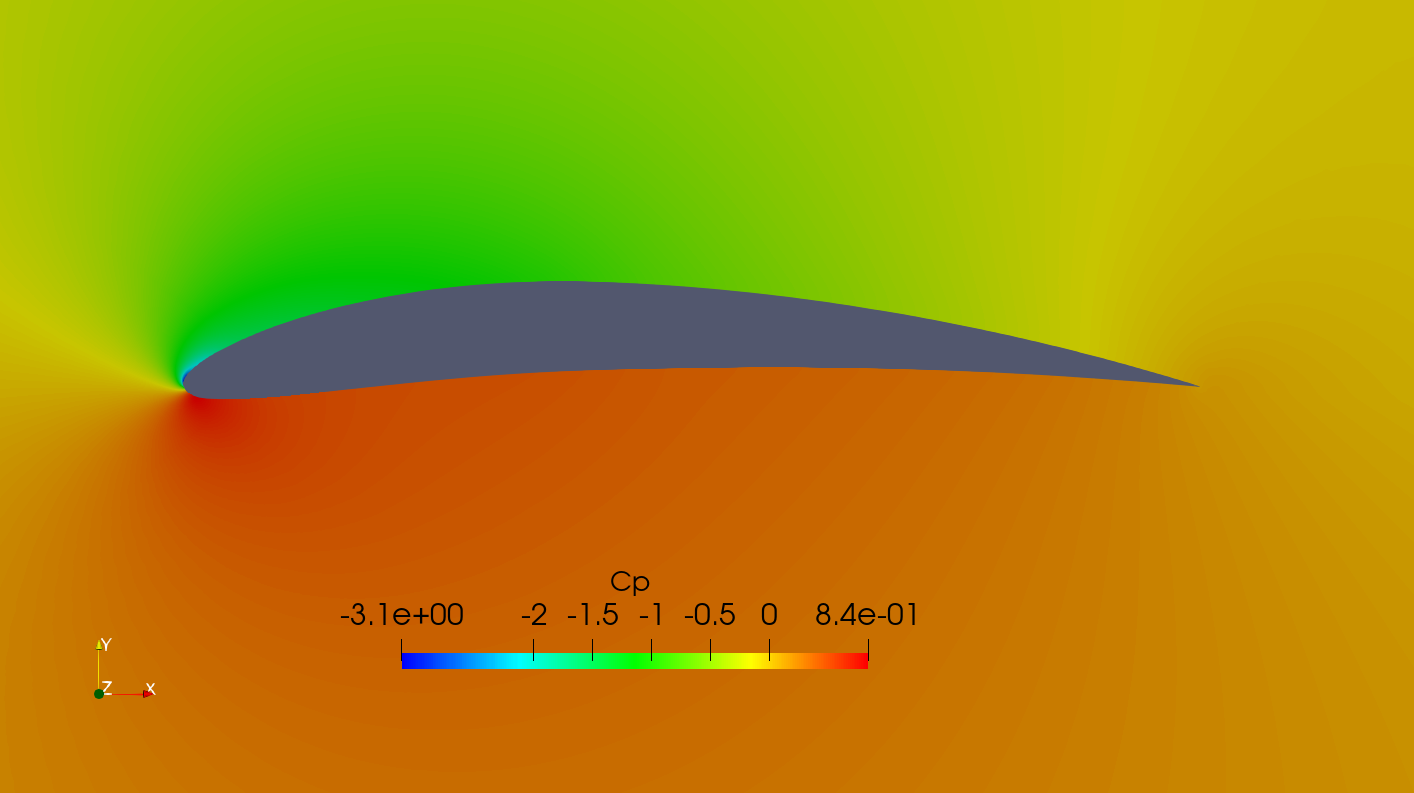
\includegraphics[width=0.4\textwidth]{Figures/CpContour.png}
    %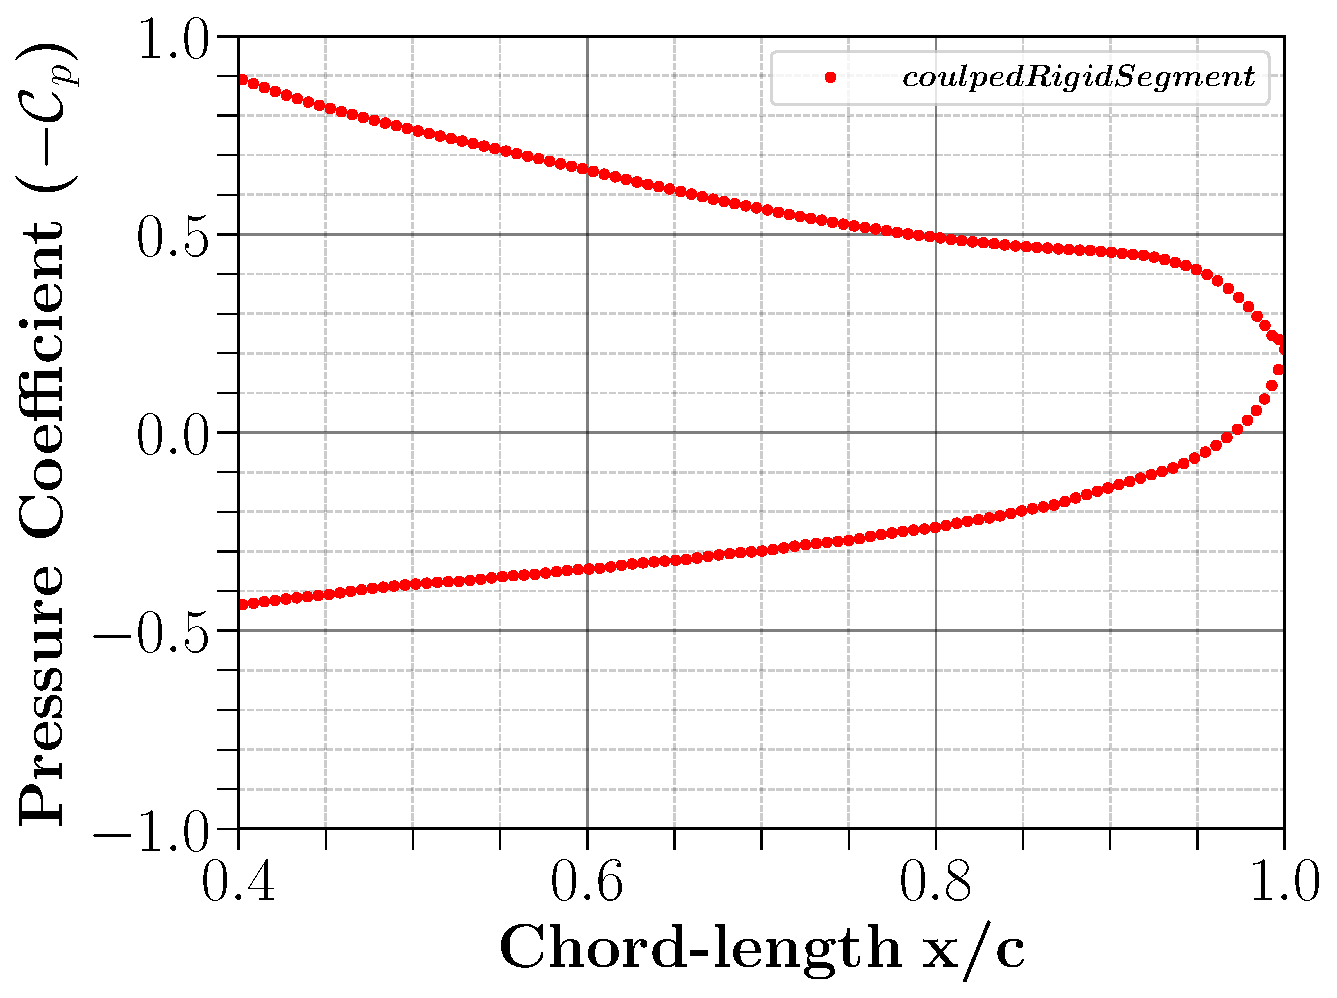
\includegraphics[width=0.42\textwidth]{figs/Cp40.pdf}
\caption{Contour of pressure coefficient at and AOA 15 using $\boldsymbol{K-\omega-SST}$}
\label{fig:Cpcontour} 
\end{figure}


\begin{figure}[ht!]
\centering
    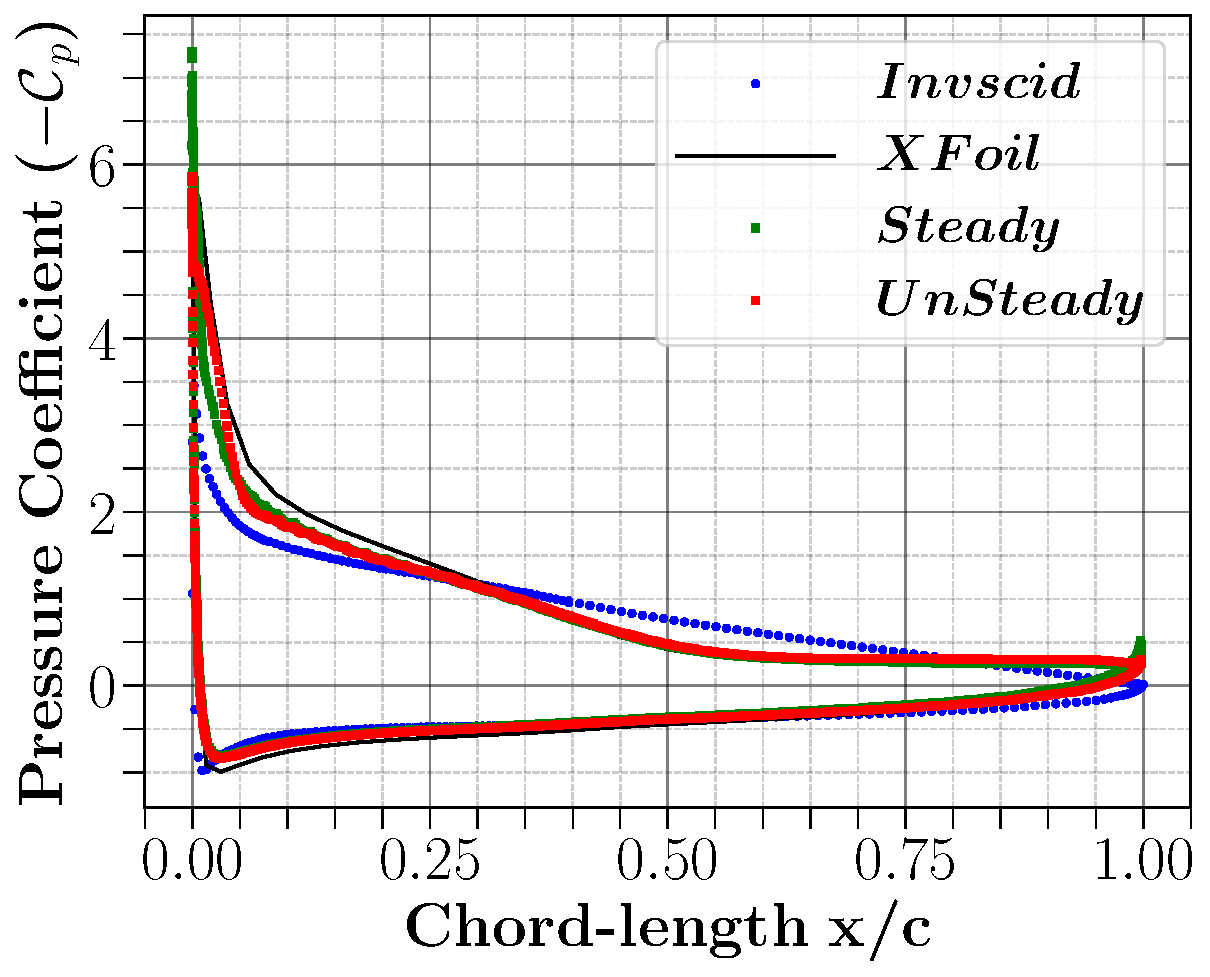
\includegraphics[width=0.4\textwidth]{figs/CfdVsXfoil.pdf}
    %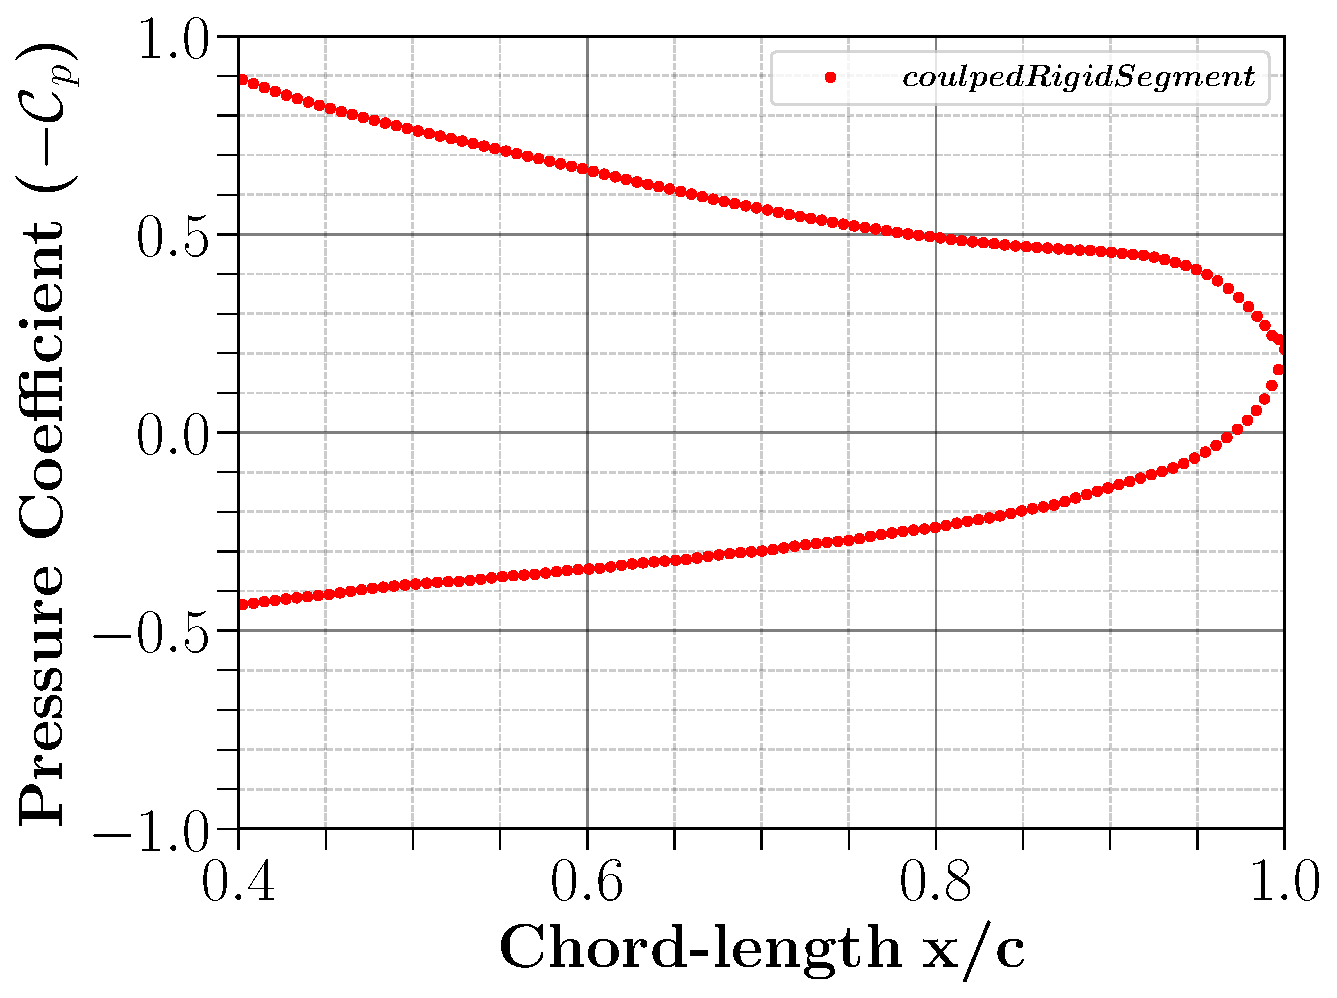
\includegraphics[width=0.42\textwidth]{figs/Cp40.pdf}
\caption{Pressure Coefficient at and AOA 15 : XFoil vs CFD}
\label{fig:Cp} 
\end{figure}




%=============================================================
\subsection{Structural Response}
\label{sec:structure}
%=============================================================


As a preliminary assessment, a constant Young's modulus can indeed be used with reasonable thicknesses along the chord.
%
The purpose is to provide a strict verification benchmark and this test case serves more for demonstration purposes.
%
The tip and airfoil trailing edge deflection (cf. Sec. \S\ref{sec:deflection}) and fluid-structure response are described in the following sections (cf. Sec. \S\ref{sec:fluidStrucutreRespnseToYoungAndRey}).

%=============================================================
\subsubsection{Tip deflection}
\label{sec:deflection}
%=============================================================

Here the results of the FSI implementation is illustrated for Young's modulus 2.5GPa and shown in Figure \ref{fig:youngEffect}.
%
The tip deflection history is shown in function of the displacements in the longitudinal direction ($\boldsymbol{D_y}$) for the tip control point on the trailing edge.
%
It illustrates the numerical computation of FSI which is performed in two stages.
%
The standard approach for coupling fluid and structural solvers is to solve the fluid dynamic equations first, then transfer the computed loads to the structural equations.
%
First the transient fluid flow is computed without coupling the fluid and structure interaction considering the whole airfoil as rigid body.
%
After the flow is developed along the wing, the system is coupled at a coupling time and takes into account the flexible segment of the airfoil.

In terms of the amount of deflection, a maximum value of deflection $10\%$ of the flexible part (we denote $\mathcal{L}$) (cf. Fig.~\ref{fig:youngEffect}).
%

However, the tip deflection is thought to remain in fluctuation motion.
%
Unlike the previous deformation, and for a Young's modulus $\mathcal{E}=2.5$ GPa, this displacement of the trailing edge tip is deflecting upwards in the same direction of the freestream velocity $\mathcal{U}_\infty$ with a maximum value of deflection $2.2\%$ of $\mathcal{L}$ (cf. Fig.~\ref{fig:airfoilSegments}).
%
The results from $\mathcal{E}=2.5$ GPa show a limited amount of fluctuations and demonstrate a state of slowdown. 


The distribution of the displacement over the flexible segment $\mathcal{L}$ grow bigger towards the wing tip owing to large displacements at the tip for both values of $\mathcal{E}$.
%
Though, the lower $\mathcal{E}$ exhibits higher tip deflection.
%
Despite the differences, these displacement distribution provide support that the high $\mathcal{E}$ generates a suddenly increase in deflection.


\begin{figure}[ht!]
\centering

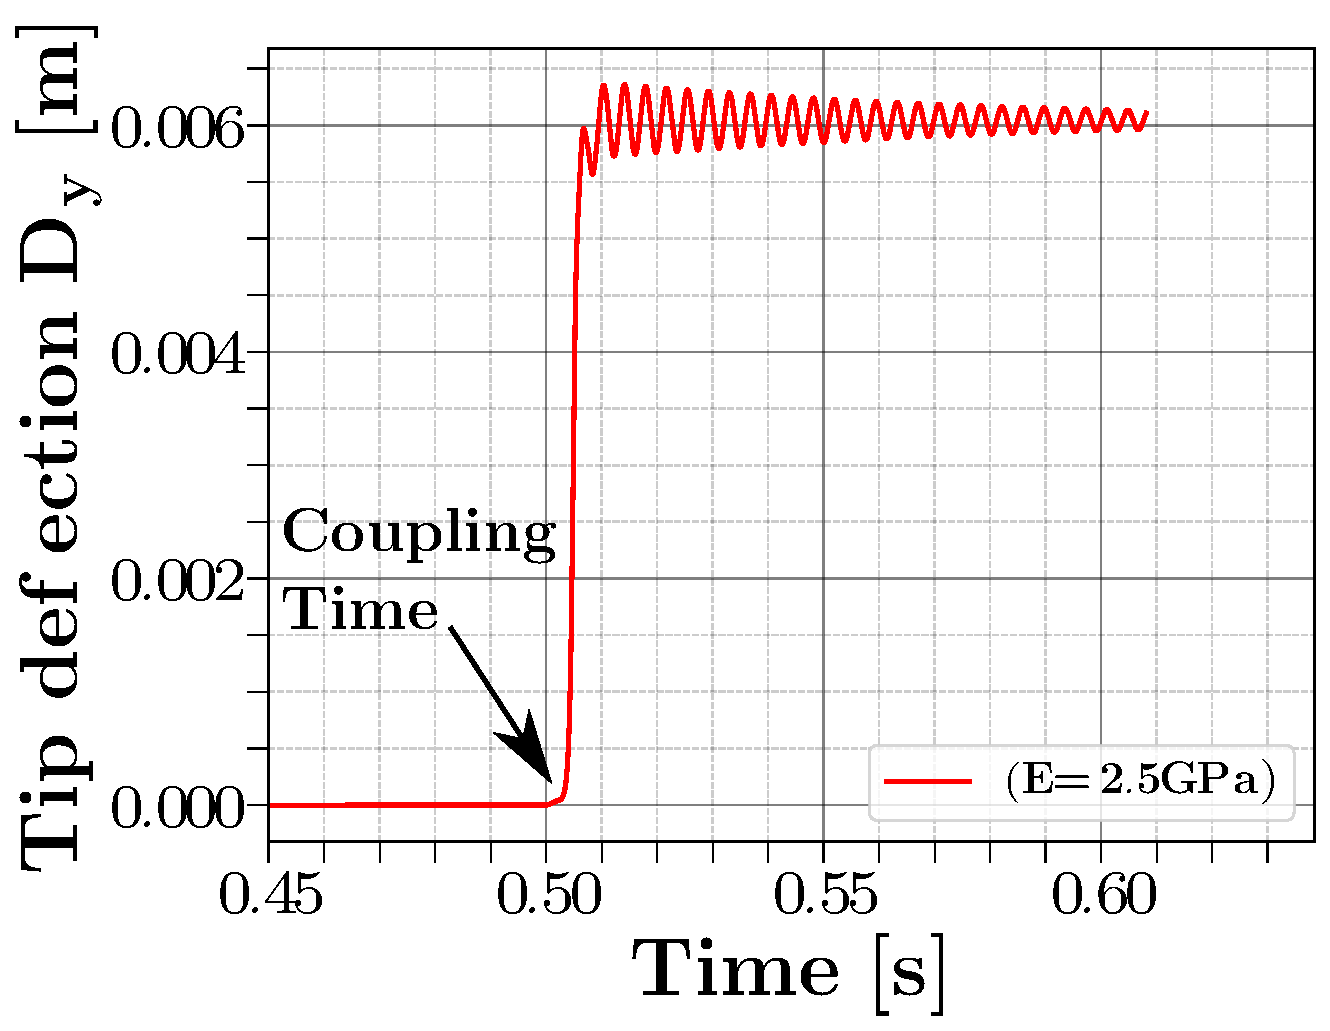
\includegraphics[width=0.5\columnwidth]{figs/deflectionvariousYoungs0.pdf}
\caption{ History of the tip displacement of the trailing edge at $\Rey =5\times10^5$ }
\label{fig:youngEffect}
\end{figure}

%
\begin{figure}[ht!]
\centering
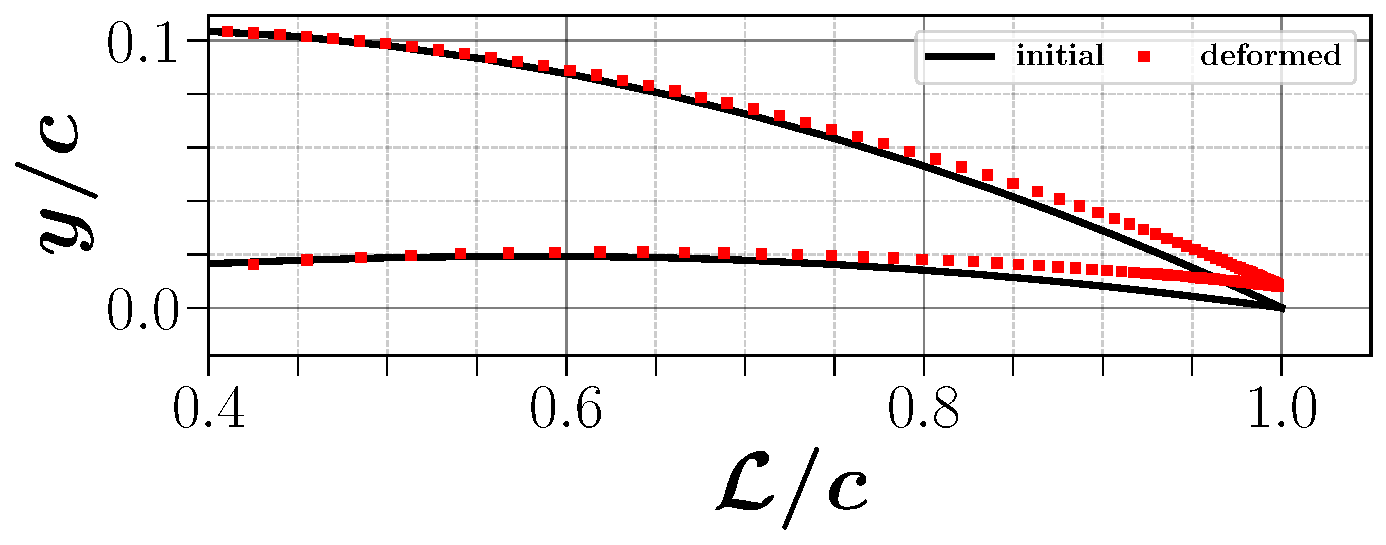
\includegraphics[width=0.50\textwidth]{figs/naca6409_deformed.pdf}
\caption{NACA6409 airfoil flexible trailing edge deflection}
\label{fig:airfoilSegments} 
\end{figure}
%

%




%


%=============================================================
\subsubsection{Fluid-structure Interaction}
\label{sec:fluidStrucutreRespnseToYoungAndRey}
%=============================================================

The computed instantaneous velocity colored streamlines are shown in Fig.~\ref{fig:25GPA} (left figure)  as well as the corresponding displacement magnitude contour of the flexible segment (right figures).
%
A small trailing edge bubble is formed and increases in diameter.
%
These separation bubbles come in a variety of sizes depending on the tip deflection.
%
For $\mathcal{E}=2.5$ GPa, it is not unexpected to see a small fluctuation of the tip and tends to be stable with the fluid flow over the flexible segment. Therefore the stable state of the tip deflection is highlighted and shows it relaxes towards steady-state structure.

Another goal of deformation control is to keep maximum wing deformation to a minimum in order to avoid damage from large stresses which is critical for control in aeroelastic applications, as it reduces material fatigue caused by vibrations and structural failures caused by high stresses.
%
The equivalent stress contour over the $\mathcal{L}$ segment and its distribution in chordwise direction are presented in Figs.~\ref{fig:stress} and \ref{fig:stress2.5GPa}, respectively.
%
The features learned from the distribution of equivalent stress over the $\mathcal{L}$ segment for $\mathcal{E}=2.5$ GPa shows promising stress relaxation with Young modulus .


%
%
\begin{figure}[ht!]
\centering
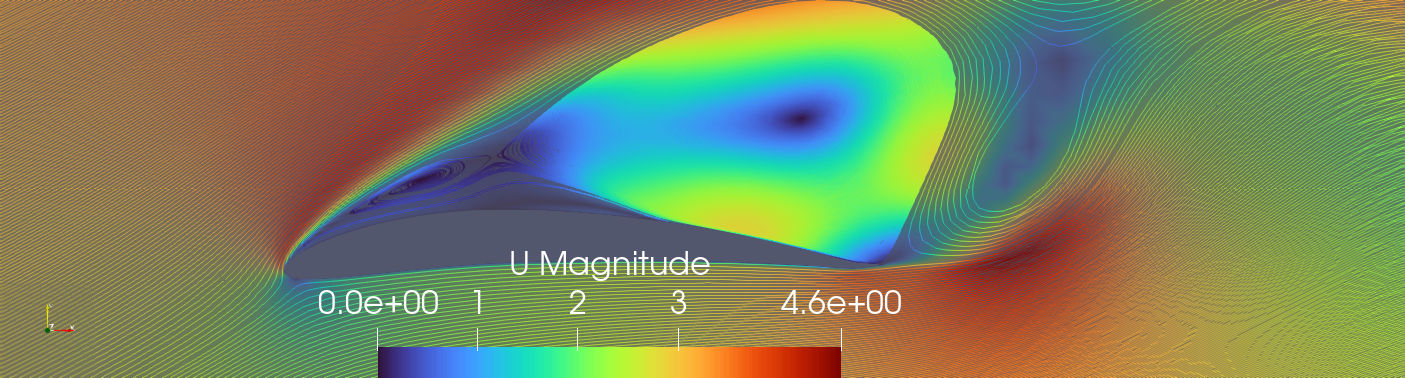
\includegraphics[width=0.45\columnwidth]{Figures/streamLines25GPACoupling.png}
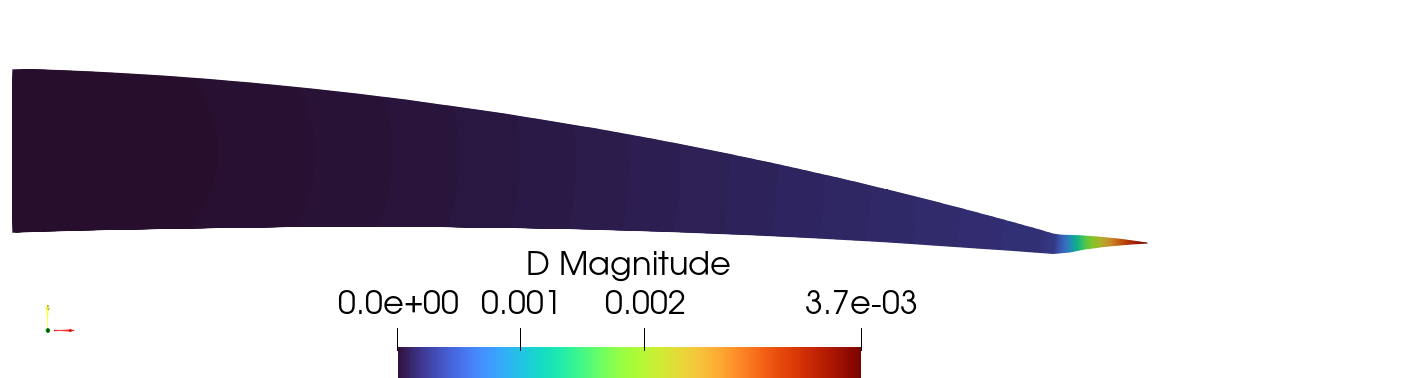
\includegraphics[width=0.45\columnwidth]{Figures/DMAgnitude25GPaCoupling.png}
\caption{Velocity colored flowfield streamlines (right) displacement contours (left) $\Rey=5\times10^5$ and $\mathcal{E}=2.5$ GPa}
\label{fig:25GPA}
\end{figure}

%
\begin{figure}[ht!]
\centering
\begin{subfigure}{.4\textwidth}
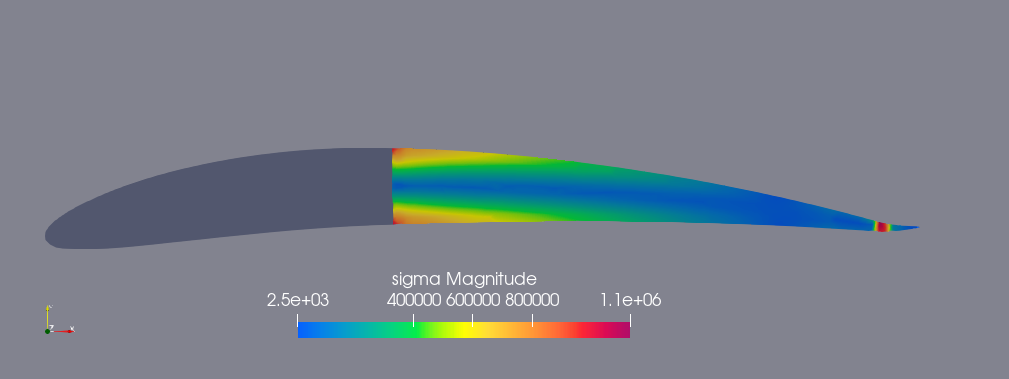
\includegraphics[width=0.99\columnwidth]{Figures/sigma.png}
\caption{\label{fig:stress} Equivalent stress contour over the flexible segment}
\end{subfigure}
\begin{subfigure}{.3\textwidth}
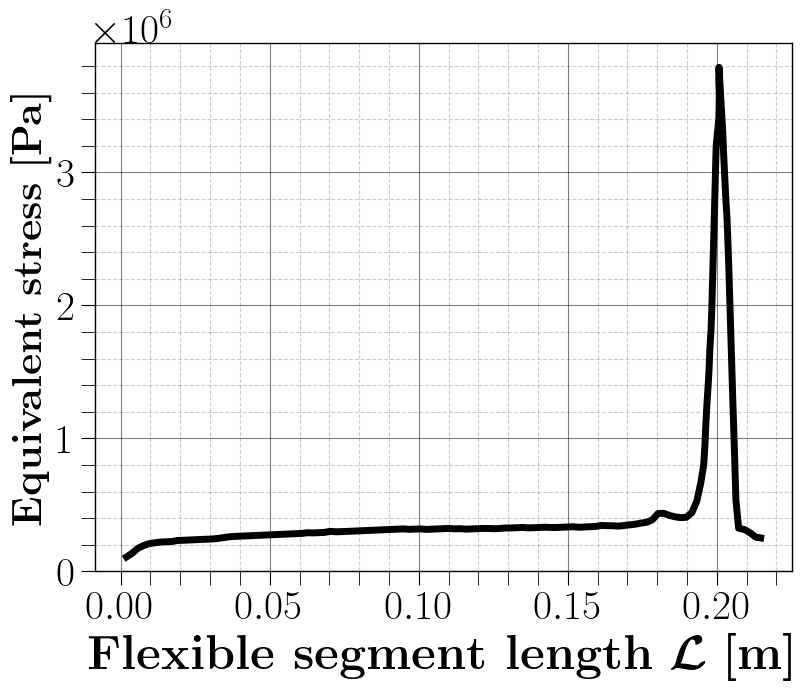
\includegraphics[width=0.99\columnwidth]{figs/equivalentstress.png}
\caption{Chordwise equivalent stress distribution\label{fig:stress2.5GPa}}
\end{subfigure}
\caption{\label{fig:displ} Stress analysis for $\mathcal{E}= 2.5$ GPa }
\end{figure}
%=============================================================
\section{Conclusion}
%=============================================================
Computational modeling can provide a way to develop predictive relationships between morphological traits and their impact on aerodynamic performance through a series of flexibility conditions will be computed using Fluid-Structure interaction (FSI).
%
In this study, we have investigated the stable FSI for turbulent conditions for bio-inspired structure requirements necessary to capture both flow field and structural analysis.
%
One of the primary objectives of evaluations is to investigate the dynamic interaction between low Reynolds number aerodynamic flow and Flexible-Biomimetic NACA6409 as earlier recommended by \citet{gamble2020b}.
%
At an angle of attack $15^{\circ}$, results of the FSI implementation are illustrated for both Young's modulus $\mathcal{E}$ of 689.5 MPa and 2.5 GPa.
%
The study highlights the importance of understanding the stable mechanical properties sufficient for biomimetic adaptive structures and materials.
%
The results suggest that $\mathcal{E}=2.5$ GPa is a promising alternative to replicate the feather and will be used in further investigation of the bird-like wings. 
%=============================================================
\section*{Acknowledgments}
%=============================================================
The Author S.B thanks Philip Cardiff collaboration for successfully implementation of Openfoam Toolbox.
%
Thanks also for Jasmin Cheuk-Máhn Wong, Lawren Gamble and Christina Harvey for fruitful discussions on the bird morphology.

This work is supported by the International University of Rabat (UIR). 
%
The authors would like to thank Imad Kissami and Simlab team for the support with the computing facilities of HPC Simlab-cluster of Mohammed VI Polytechnic University at Benguerir (UM6P).
